% ==============================================================================
% siamart.cls loads breakurl (dvips-only; breaks under XeTeX/tectonic)
% whenever it is not running under pdfTeX. Mark breakurl as already
% loaded so the class's \RequirePackage is a no-op; XeTeX's own
% hyperref driver breaks links natively.
\expandafter\def\csname ver@breakurl.sty\endcsname{2013/04/10 v1.40 stub}
\documentclass[hidelinks]{siamart}

% Packages beyond those provided by siamart.cls (which loads amsmath,
% ntheorem, hyperref, algorithm, xcolor)
\usepackage{mathtools}
\usepackage{amssymb}
\usepackage{booktabs}
\usepackage{multirow}
\usepackage{multicol}
\usepackage{graphicx}
\usepackage{comment}

% Theorem-like environments not predefined by the class (theorem, lemma,
% corollary, proposition, definition, proof are provided by siamart)
\newsiamremark{remark}{Remark}
\newsiamthm{condition}{Condition}
% Unnumbered environment for the informal statement of the main result.
\theoremstyle{nonumberplain}
\theoremheaderfont{\normalfont\sc}
\theorembodyfont{\normalfont\itshape}
\theoremseparator{.}
\theoremsymbol{}
\newtheorem{mainresult}{Main result}
\numberwithin{theorem}{section}
\providecommand{\qedhere}{}     % ntheorem places the end-of-proof mark itself

\title{Operator-adapted preconditioners for the conjugate-gradient method}
% TODO: working title. Alternates carried from main_abridged.tex.
\author{Obed Camacho\thanks{Institute for Computational and Mathematical
    Engineering, Stanford University (\email{obedc@stanford.edu}).}
  \and
  Adrian Lew\thanks{Department of Mechanical Engineering and Institute for
    Computational and Mathematical Engineering, Stanford University
    (\email{lewa@stanford.edu}).}}
% TODO: author order, funding \thanks on the title.
\headers{Operator-adapted preconditioners for the conjugate-gradient method}{O.~Camacho and A.~Lew}
% TODO: confirm the shortened running head above.

\begin{document}
\maketitle

\begin{abstract}
The operator-adapted wavelet (OAW) factorization is a sparse approximate
inverse factorization for the stiffness matrices of second-order elliptic
PDEs whose quasi-linear complexity and provable
accuracy guarantees with $L^\infty$ coefficients make it an attractive
method for solving multiscale problems. However, the method's use as a direct solver has confined it to moderate problem sizes. We prove that the factorization may
instead serve as a preconditioner for the conjugate gradient method and quantify the rate of convergence. For a
problem with $N$ degrees of freedom and error tolerance $\varepsilon$, this
reduces the setup cost from $\mathcal{O}(N\ln^{2d+1}(N/\varepsilon))$ to
$\mathcal{O}(N(\ln\ln N)^{2d})$ (independent of $\varepsilon$) and the solution cost
from $\mathcal{O}(N\ln^{d+1}(N/\varepsilon))$ to
$\mathcal{O}(N(\ln\ln N)^{d}\ln(1/\varepsilon))$. We further control the memory demands of
the algorithm by solving subproblems iteratively rather than with stored
factorizations, storing the preconditioner in a compressed factored form, and exploiting available problem symmetries, whereby the method thereby extends to large-scale systems. We demonstrate this on three-dimensional diffusion and elasticity problems with $N \gtrsim 10^{6}$ degrees of freedom on a single
GPU, and compare with standard algebraic multigrid solvers.
\end{abstract}

\begin{keywords}
  operator-adapted wavelets, gamblets, preconditioner, multigrid, GPU,
  rough coefficients
\end{keywords}
% TODO: review keywords.

\begin{AMS}
  65N55, 65F08, 65N30
\end{AMS}
% TODO: review AMS subject classifications.

% ==============================================================================
% Skeleton generated from paper/BLUEPRINT.md. Each BP comment marks the
% landing site of one blueprint bullet; content lands per the harvest
% manifest (paper/HARVEST_MANIFEST.md) or is drafted fresh.
% ==============================================================================

\section{Introduction}
\label{sec:intro}








We consider elliptic variational problems of the form
\begin{equation}\label{eq:general_problem}
  u\in\mathcal V,\qquad
  a(u,v)=\ell(v)\quad\text{for all }v\in\mathcal V,
\end{equation}
where $\mathcal{V} \subseteq H^s(\Omega)$ a Sobolev space, $\Omega$ is a bounded piecewise-Lipschitz domain, $a$ is a bounded, symmetric, coercive, and local bilinear form, and boundary conditions are incorporated into the choice of trial space and load functional $\ell$. This setting includes, for example, diffusion--reaction and linear elasticity problems. A conforming finite-element discretization yields a symmetric positive definite system
\begin{equation}\label{eq:linear_system}
Ku = g.
\end{equation}
over a finite-dimensional trial space $\mathcal{V}^{(q)} \subset\mathcal{V}$ of
dimension~$N$,


\iffalse
We consider boundary-value problems of the form
\begin{equation}\label{eq:general_problem}
  \mathcal{L}\mathbf{u} \;=\; g,
  \quad \mathcal{B}u = h,
\end{equation}
where $ \mathbf{u}\in \mathcal{V} \subseteq W^{s,2}_0(\Omega)$, a Sobolev space over a
bounded Lipschitz domain $\Omega \subset \mathbb{R}^d$, $  \mathcal{L} : \mathcal{V} \to \mathcal{V}^{*}$ is a
linear, bounded, symmetric, and coercive differential operator with coefficients in $L^{\infty}$, and $\mathcal{B}:\mathcal{V} \to \mathcal{V}$ is an operator specifying the appropriate boundary conditions. We further stipulate that the bilinear form
$a(\mathbf{u},\mathbf{v}) := [\mathcal{L}\mathbf{u}, \mathbf{v}]$ be \emph{local}, in the sense of being induced by an
integrable energy density on~$\Omega$. Our hypotheses ensure existence, uniqueness, and continuous dependence of the solution $\mathbf{u}$ on the data~\cite{ErnGuermond2004}, and are satisfied by many physically relevant problems, such as diffusion-reaction or elasticity. A conforming finite-element discretization of \eqref{eq:general_problem} solves the weak form,
\begin{equation}\label{eq:weak_form}
  a(u,v) \;=\; \ell_g(v)
  \qquad \forall\, v \in \mathcal{V}^{(q)},
\end{equation}


over a finite-dimensional trial space $\mathcal{V}^{(q)} \subset\mathcal{V}$ of
dimension~$N$, where $\ell_g \in \mathcal{V}^{(q)*}$ encodes the right-hand side $g$ and boundary conditions $\mathcal{B}$. Choosing a finite-element basis for $\mathcal{V}^{(q)}$ yields a sparse symmetric positive definite (SPD) system
\begin{equation}\label{eq:linear_system}
Ku = g.
\end{equation}


Coercivity is inherited by the conforming subspace, so the discrete problem is well posed.
\fi

Solving this linear system is a fundamental task in computational physics and engineering. For small systems this may be done directly through dense factorizations, but such techniques become computationally infeasible as $N$ grows. Sparse direct factorizations (such as sparse LU or Cholesky) scale better for larger systems, but their cost in work and memory still grows superlinearly in~$N$~\cite{golub2013matrix}.%
\footnote{TODO: cite nested-dissection complexity.}
Because of this, iterative methods are often preferred at scale. For SPD systems the standard choice is the conjugate gradient method (CG), whose iteration count scales with $\sqrt{\kappa(K)}$, the condition number of~$K$~\cite{saad2003iterative}. On a quasi-uniform mesh, $\kappa(K)$ grows as $N^{2/d}$, with a prefactor depending on the coefficient contrast~\cite{ErnGuermond2004}, so the iteration count scales as $N^{1/d}$ and a preconditioner must typically be employed to make CG practical. Among the most widely used preconditioners for SPD linear systems with multiple length scales are the geometric and algebraic
multigrid methods (GMG and AMG, respectively), whose nominal solve time and memory are near-linear in~$N$. As Brannick et al. observe, constructing or enforcing the hypotheses required to obtain this optimal rate is of at least quadratic complexity in~$N$, incompatible with the desired linear complexity~\cite{brannick2019role}. In particular, a basis for the optimal coarse space may be constructed by minimizing the $K$-energy of each basis function while imposing a set of interpolation constraints, but the minimizers are globally supported and the associated coarsening matrices are dense. Practice circumvents this tension with coarsening and smoothing heuristics, such as smoothed aggregation schemes\cite{saad2003iterative} or approximate energy-minimizing interpolation under imposed sparsity \cite{Wan1998EnergyMinimizing}.

As a result, obtaining good convergence on a given problem often requires extensive tuning and domain-specific knowledge, particularly when the coefficients are non-smooth and vary over a wide range of length scales. However, a hierarchy of bases for \emph{approximate} orthogonal coarse spaces may be constructed at near-linear cost via the operator-adapted wavelet (OAW) decomposition of Owhadi~\cite{owhadi2017,Owhadi_Scovel_2019}. Bases for these spaces are constructed recursively from the full trial space via the same energy-minimizing principle as above, yielding a basis in which the operator becomes block diagonal, with one uniformly well-conditioned block per length scale. The globally supported basis functions are provably well approximated by functions with prescribed support on compact \emph{patches} in $\Omega$, with an error decaying exponentially in the radius $\rho$ of the support patch. The result is an approximate factorization of $K^{-1}$ with sparse factors, quasi-linear complexity, and rigorous accuracy guarantees for general $L^\infty$ coefficients. 
%[TODO: mention the LOD or Peterseim as similar constructions, other direct multilevel methods, typically used for homogenization]
%[TODO: a figure would be helpful here]

The error in the solution obtained from this direct factorization is bounded by the choice of localization. More precisely, with localization radius $\rho$, the preprocessing cost scales as $\mathcal{O}(N\rho^{3d})$ in time, and the stored hierarchy grows as $\mathcal{O}(N\rho^{d})$ in memory~\cite{owhadi2017}. Ensuring a prescribed relative energy-norm error tolerance $\varepsilon$ requires $\rho \sim \ln(N/\varepsilon)$, resulting in $\mathcal{O}(N\ln^{3d}(N/\varepsilon))$ time and $\mathcal{O}(N\ln^{d}(N/\varepsilon))$ memory cost, and obtaining an approximate solution with the stored factorization has cost $\mathcal{O}(N\ln^{d+1}(N/\varepsilon))$. Improving the accuracy of the solution or perturbing the operator $a$ therefore requires repeating the comparatively expensive preprocessing with larger $\rho$. This is particularly limiting for implicit time-stepping problems; Owhadi and Zhang~\cite{owhadi_tpde} note that for heterogeneous time-steps, a change of step size repeats the full preprocessing cost, while Chen et al.~\cite{chen2021} observe the accumulation of approximation errors over time-steps if one does not incorporate post-hoc correction techniques. Existing realizations also assemble and store large global objects: the fine-scale stiffness matrix, the change of basis from nodal to OAW coordinates, and sparse-direct factorizations of the diagonal blocks, all of which strain working memory and storage constraints if one attempts to scale the algorithm naively. These costs have confined published implementations to moderate problem sizes, despite the nominally near-linear cost of the OAW factorization.

% BP: related work beyond the OAW line (robust multigrid and domain
%     decomposition for heterogeneous coefficients; hierarchical
%     factorization lines) -- content TODO, single home per comparison.

Many of these limitations are consequences of deploying the factorization as a direct approximate inverse, and while using the hierarchy as a preconditioner is noted as a possibility in~\cite{owhadi2017}, this direction is neither analyzed nor implemented there. A stored factorization with sparse-LU diagonal blocks was applied
heuristically in~\cite{sik2025hfm} to precondition a two-dimensional
electromagnetic model problem, but without supporting analysis or an
implementation scaling to larger problems in three dimensions.  In this paper, we provide this missing analysis and address barriers to scalability of the OAW transform. We focus on using this factorization as a preconditioner for the conjugate gradient method, decoupling accuracy requirements from the build time and memory demands and allowing more aggressive approximation of local problems while preserving convergence guarantees. We provide explicit bounds on the condition number of the preconditioned system as a function of the problem size $N$ and the localization radius $\rho$. These bounds imply that CG convergence to arbitrary tolerance may be obtained in a number of iterations bounded independently of $N$, by taking a localization radius scaling asymptotically as $\ln \ln N$.

The main technical ingredient in this result is a bound on the pairwise energy interactions of the localization errors (Lemma~\ref{lem:error_interactions}), which
reduces the naive estimate on $\kappa$ by a factor of $\sqrt{N}$. Due to exponential decay of the basis functions for the coarse spaces, the errors in the exponential tails of the basis functions are approximately orthogonal in the energy norm, and this, combined with their exponential smallness, tightens the bound. We also show that the same factorization may precondition a \emph{perturbed} operator, and quantify the resulting increase in the iteration count. In particular, a single hierarchy may be used across every step of a variable-time-step time-stepping scheme, addressing a limitation of~\cite{owhadi_tpde} and~\cite{chen2021}. 

We also present a practical algorithm to reduce demands on working memory and storage, allowing the construction to be feasible in three dimensions for $N \gtrsim 10^6$. 
We first observe that the sparsity patterns of the matrices in the algorithm may be computed a-priori from the mesh geometry, allowing for the efficient allocation of memory 
and reducing the number of matrix indices that need to be stored in memory. The storage demands of the coarsening operators may also be substantially reduced by exploiting local translation
symmetries. Further savings may be achieved during preprocessing by solving local problems \emph{iteratively} in parallel batches and by using only the action $x \mapsto Kx$, rather than
assembling $K$ explicitly, where possible.

The remainder of the paper is structured as follows.
Section~\ref{sec:results} states the main results: the setting and
definitions, the conditioning and cost guarantees, and the algorithms as
implemented.  Section~\ref{sec:construction} develops the construction:
its sparsity structure, storage scheme, and symmetry compressions.
Section~\ref{sec:preconditioner} contains the analysis.
Section~\ref{sec:experiments} reports experiments and scaling behavior
for high-contrast scalar diffusion and linear elasticity on a single A100
GPU, comparing with prior OAW implementations and AMG baselines.  In
Section~\ref{sec:conclusions} we make some concluding remarks, indicating
the limitations of our analysis as well as directions for future work.
The OAW factorization is reviewed from first principles in
Appendix~\ref{app:oaw}.
% TODO: finalize the experiment list once experiments are regenerated.

\section{Background}
\label{sec:background}

We establish the notation required to state the main results and review some of the relevant work of~\cite{Owhadi_Scovel_2019}, to which we refer the reader for a complete treatment of OAW theory. 
%primitive objects
\subsection{Exact Basis Construction}
We retain the setting and notation of~\eqref{eq:general_problem} and ~\eqref{eq:linear_system}. Fix an integer $q > 1$ and let $\mathcal{V}^{(q)}
\subset \mathcal{V}$ be a conforming finite-element trial space of dimension
$n_q := N$ on a mesh of width~$h_q$, with respect to which the stiffness matrix of~$a$ is~$K$. We introduce a nested hierarchy of sets of linearly
independent \emph{measurement functionals} $\{\mu^{(k)}_j\}_{j=1}^{n_k} \subset (\mathcal{V}^{(q)})^*$,
$k = 1,\ldots,q$
\begin{equation}\label{eq:measurement_nesting}
  \mathcal{V}^{(k)*} := \operatorname{span}\{\mu^{(k)}_j\}_{j=1}^{n_k}
  \;\subset\; \mathcal{V}^{(k+1)*}.
\end{equation}
The nesting is encoded by matrices $C^{(k)} \in \mathbb{R}^{n_k \times n_{k+1}}$, $1 \leq k < q$,
\begin{equation}\label{eq:nesting_maps}
  \mu^{(k)}_i = \sum_{j=1}^{n_{k+1}} C^{(k)}_{ij}\,\mu^{(k+1)}_j,
  \qquad 1 \leq i \leq n_k,
\end{equation}
and we fix a parameterization $D^{(k)} \in \mathbb{R}^{d_k \times n_{k+1}}$, $1 \leq k < q$,
$d_k := n_{k+1} - n_k$, of the right kernel of~$C^{(k)}$:
\begin{equation}\label{eq:kernel_D}
  C^{(k)}\, D^{(k)\top} = 0,
  \qquad \operatorname{rank} D^{(k)} = d_k.
\end{equation}
In this convention level~$q$ is the finest (trial-space) mesh, and we assume the coarser spaces are obtained via uniform coarsening with coarsening ratio $H \in (0,1)$; $h_{k-1} = \frac{h_{k}}{H}$. Throughout, the level-$k$ functionals $\mu^{(k)}_j$ are assumed to be in
one-to-one correspondence with the degrees of freedom of a shape-regular FEM
mesh of width $h_k \propto H^k$. Each functional is associated with a node~$x^{(k)}_j$ and supported on a union of $\mathcal{O}(1)$ cells about this node (this ensures sparsity of the linear systems).
This gives $n_k \propto  h_k^{-d}$, so each coarsening step reduces the
dimension by the factor $H^{d}$ and $q \leq C_q(H,d) \ln N$. \footnote{We further assume throughout that the hierarchy satisfies the stability conditions of~\cite{Owhadi_Scovel_2019}, restated here in Appendix~\ref{app:stability}.  These have been verified for three families of
measurement functionals: normalized cell indicators (Haar prewavelets),
local polynomials, and subsampled
Dirac deltas with regularity $s > d/2$~\cite[\S14.8, Thms.~16.38--16.39]{Owhadi_Scovel_2019}.} 

% The exact basis
The measurement functionals are used to define a multi-resolution basis of the trial space
$\mathcal{V}^{(q)}$ organized by the levels of the measurement
hierarchy as follows:
For $1 \leq i \leq n_k$,
define the affine feasible set
\begin{equation}\label{eq:constraint_set}
  \mathcal{A}^{(k)}_i
  := \{v \in \mathcal{V}^{(q)} : \mu^{(k)}_j(v) = \delta_{ij},\;
       1 \leq j \leq n_k\},
\end{equation}
the level-$k$ basis function is
\begin{equation}\label{eq:psi_k_def}
    \psi^{(k)}_i = \operatorname{argmin}_{f \in \mathcal{A}^{(k)}_i} \lVert f\rVert_a \, .
\end{equation}
$\mathcal{A}^{(k)}_i$ is nonempty and affine and the energy norm is
strictly convex, so a unique minimizer exists.  \footnote{These functions
are also called \emph{gamblets}, after the game-theoretic derivation
in~\cite{owhadi2017}.}  $\mathcal{V}^{(k)} := \operatorname{span}\{\psi^{(k)}_i\}_{i=1}^{n_k}$ is the level $k$ \emph{coarse space}.~\eqref{eq:measurement_nesting} implies the nesting,
$\mathcal{V}^{(k)} \subset \mathcal{V}^{(k+1)}$
\footnote{See Appendix~\ref{app:oaw} for a proof}. We then define the level-$k$ \emph{detail space} $\mathcal{W}^{(k)}$ to be the
$a$-orthogonal complement of $\mathcal{V}^{(k)}$ in
$\mathcal{V}^{(k+1)}$, of dimension $d_k = n_{k+1} - n_k$.  
A decomposition for the trial space is then obtained recursively:

\begin{equation}\label{eq:scale_decomposition}
  \mathcal{V}^{(k+1)} = \mathcal{V}^{(k)} \oplus_a \mathcal{W}^{(k)},
  \qquad
  \mathcal{V}^{(q)} = \mathcal{V}^{(1)} \oplus_a \mathcal{W}^{(1)}
  \oplus_a \cdots \oplus_a \mathcal{W}^{(q-1)} ,
\end{equation}
Bases for the $\mathcal{W}^{(k)}$ (termed \emph{detail functions}) can be defined
recursively as\footnote{See Appendix~\ref{app:oaw} for a proof that these
form bases of the detail spaces.}
\begin{equation}\label{eq:detail_basis}
  \chi^{(k)}_j = \sum_{m=1}^{n_{k+1}} D^{(k)}_{jm}\,\psi^{(k+1)}_m,
  \qquad 1 \leq j \leq d_k .
\end{equation}
%In particular, the detail functions are $a$-orthogonal to the coarse
%space $\mathcal{V}^{(k)}$: by first-order optimality
%in~\eqref{eq:psi_k_def}, $a(\psi^{(k)}_i, v) = 0$ for every trial
%function $v$ whose level-$k$ measurements vanish, and the level-$k$
%measurements of the $\chi^{(k)}_j$ vanish by~\eqref{eq:nesting_maps}
%and~\eqref{eq:kernel_D}.

By~\eqref{eq:scale_decomposition}, the $n_1 + d_1 + \cdots + d_{q-1} = n_q$ functions
\begin{equation}\label{eq:combined_basis}
  \varphi_i :=
  \begin{cases}
    \psi^{(1)}_i, & 1 \leq i \leq n_1, \\[2pt]
    \chi^{(k)}_{\,i - n_k}, & n_k < i \leq n_{k+1}, \quad 1 \leq k < q,
  \end{cases}
\end{equation}
form a basis of $\mathcal{V}^{(q)}$, ordered from the coarsest scale to
the finest.  We denote by $\Phi$ the invertible matrix whose $i$-th
column holds the coefficients of $\varphi_i$ in the fine-mesh finite-element basis. % Block diagonalization and the exact inverse
The components of the stiffness matrix of~$a$ in this basis are
$G_{ij} = a(\varphi_i, \varphi_j)$, i.e. $G = \Phi^\top K \Phi$. By $a$-orthogonality of the summands in~\eqref{eq:scale_decomposition},
$G$ is \emph{block diagonal}:
\begin{equation}\label{eq:block_diagonal}
  G = \operatorname{diag}\bigl(B^{(1)}, B^{(2)}, \ldots, B^{(q)}\bigr) := D,
\end{equation}
with $B^{(1)}_{ij} = a(\psi^{(1)}_i, \psi^{(1)}_j)$ and
$B^{(k)}_{ij} = a(\chi^{(k-1)}_i, \chi^{(k-1)}_j)$ for $k \geq 2$.  The
blocks are uniformly well conditioned
\cite[Thm.~14.17]{Owhadi_Scovel_2019}:
\begin{equation}\label{eq:block_conditioning}
  C_B^{-1}\, H^{-2(k-1)}
  \;\leq\; \lambda_{\min}\bigl(B^{(k)}\bigr)
  \;\leq\; \lambda_{\max}\bigl(B^{(k)}\bigr)
  \;\leq\; C_B\,H^{-2k},
\end{equation}
where $C_B$ depends on $a$ but not on $N$ or the mesh (Appendix~\ref{app:stability}), so that
$\kappa(B^{(k)}) \leq C_B^2 H^{-2}$ for every $k$.  Since $\Phi$ is invertible,
\begin{equation}\label{eq:exact_inverse_formula}
  K^{-1} = \Phi\, G^{-1}\, \Phi^\top
         = \Phi \operatorname{diag}\bigl(B^{(k)\,-1}\bigr) \Phi^\top .
\end{equation}
Applying the inverse through~\eqref{eq:exact_inverse_formula} is then a
restriction by $\Phi^\top$, one independent, well conditioned solve per diagonal block,
and a prolongation by~$\Phi$.  


\subsection{Localized Basis}\label{subsec:loc}
The basis functions $\psi^{(k)}_i$ and $\chi^{(k)}_j$ are globally
supported, so the change of basis $\Phi$ and the blocks $B^{(k)}$ are
dense, making the exact construction computationally infeasible for large $N$. We associate with $\psi^{(k)}_i$ the node $x^{(k)}_i$ associated with the sole non-zero measurement constraint in~\eqref{eq:psi_k_def}. The energy of $\psi^{(k)}_i$ decays
exponentially with distance from~$x^{(k)}_i$, with decay length
proportional to the mesh width of the
level~\cite[Thm.~15.41]{Owhadi_Scovel_2019}.
% Localization
This exponential decay motivates the definition of the \emph{localized basis functions}
$\psi^{(k)}_{\rho,i}$: fix $\rho > 0$
and let $S^{(k)}_i$ be a union of mesh cells contained in a ball of radius $\rho h_k$
and containing the support of $\mu^{(k)}_i$, such that the interior of $\operatorname{supp} \mu^{(k)}_j$ does not intersect the boundary of~$S^{(k)}_i$ for any $j$. Then define %Appendix~\ref{app:stability} realizes such a choice for each measurement family.
\begin{equation}\label{eq:localized_constraint_set}
  \mathcal{A}^{(k)}_{\rho,i}
  := \bigl\{ v \in \mathcal{V}^{(q)} :
     \operatorname{supp} v \subseteq S^{(k)}_i,\;
     \mu^{(k)}_j(v) = \delta_{ij} \text{ for every } j \text{ with }
     \operatorname{supp} \mu^{(k)}_j \subseteq S^{(k)}_i \bigr\} ,
\end{equation}
\begin{equation}\label{eq:localized_basis}
  \psi^{(k)}_{\rho,i}
  := \operatorname{argmin}_{f \in \mathcal{A}^{(k)}_{\rho,i}}
     \lVert f \rVert_a .
\end{equation}
Since the patch has radius $\rho h_k$ on a mesh
of width~$h_k$, each patch contains $\mathcal{O}(\rho^d)$
level-$k$ degrees of freedom.

The minimizer over the patch approximates the exact basis function with
an error exponentially small in the patch radius
\cite[Thm.~15.41]{Owhadi_Scovel_2019}: writing $r_k := \rho h_k$ for the
physical radius of the patch,
\begin{equation}\label{eq:localization_error}
  \|\psi^{(k)}_i - \psi^{(k)}_{\rho,i}\|_a
  \;\leq\;
  C\,\|\psi^{(k)}_i\|_a\;e^{-r_k/(2\ell h_k)} ,
\end{equation}
with $C$ depending on the operator but not on $k$ or the radius, and
$\ell$ a dimensionless constant depending only on the continuity and coercivity constants of $a$.
% Both estimates are stated in relative form: the h^{-s} prefactors of
% [OS2019, Thm. 15.41] equal ||psi_i||_a up to constants by
% [OS2019, Lemma 15.43, (15.132)].
% eq:localized_basis poses the local problem over a patch contained in the
% radius-rho h_k ball of [OS2019, Thm. 15.41]; the difference is absorbed
% into C.
% The chi estimates are not stated in OS2019; combination argument
% (D-row locality, C_mu bounds, norm ratio ~ H^{-1}).
% OS2019 Ch. 15 absorbs the coefficient contrast into its constants; no
% explicit contrast formula is stated. The worst-case ell ~ sqrt(contrast)
% stays cited to the model setting of owhadi2017.
The localized detail functions are defined as
\begin{equation}\label{eq:localized_detail_basis}
  \chi^{(k)}_{\rho,j}
  = \sum_{m=1}^{n_{k+1}} D^{(k)}_{jm}\,\psi^{(k+1)}_{\rho,m},
  \qquad 1 \leq j \leq d_k .
\end{equation}
Estimates analogous to \eqref{eq:localization_error} hold for the $\chi^{(k)}_j$ and
$\chi^{(k)}_{\rho,j}$, with constant prefactors depending on~$D^{(k)}$.
% The localized factorization and the preconditioner 
Concatenating the localized functions in the same order as ~\eqref{eq:combined_basis} yields the localized multiresolution basis
$\varphi_{\rho,i}$, and we write $\Phi_\rho$ for the invertible matrix whose
$i$-th column holds the coefficients of $\varphi_{\rho,i}$ in the
fine-mesh basis. Define the \emph{localized}
stiffness matrix
\begin{equation}\label{eq:G_rho}
  G_{\rho} \;=\; \Phi_{\rho}^{\top} K \, \Phi_{\rho},
\end{equation}
with entries $G_{\rho,ij} = a(\varphi_{\rho,i}, \varphi_{\rho,j})$.
Inverting the congruence gives
\begin{equation}\label{eq:exact_identity}
  K^{-1} \;=\; \Phi_{\rho}\, G_{\rho}^{-1}\, \Phi_{\rho}^{\top}.
\end{equation}
Unlike~$G$, $G_\rho$ is
not in general block diagonal; we write
\begin{equation}\label{eq:gram_split}
  G_\rho \;=\; D_\rho + E_\rho,
\end{equation}
where $D_\rho = \operatorname{diag}\{B^{(k)}_{\rho}\}_{k=1}^{q}$ is the
block-diagonal part, the blocks defined as in~\eqref{eq:block_diagonal}
from the localized functions, and $E_\rho := G_\rho - D_\rho$ consists
of the blocks coupling different levels. Note that $G_\rho$ is SPD by congruence to~$K$, and since each $B^{(k)}_\rho$ is a principal submatrix of~$G_\rho$, so is
$D_\rho$. The off-diagonal couplings $E_{\rho}$ are not typically constructed, and the
inverse is then approximated as
\begin{equation}\label{eq:preconditioner}
  \widetilde{K}_{\rho}^{-1}
  \;=\; \Phi_{\rho}\,D_{\rho}^{-1}\,\Phi_{\rho}^{\top}.
\end{equation}
Constructing these factors requires $\mathcal{O}(N\rho^{\alpha d})$ time and
working memory (where $\alpha \in (1, 3)$ depends on the method used to
solve the localized optimizations \ref{eq:localized_basis}), storing the factors costs
$\mathcal{O}(N\rho^d)$ space, and the matrix-vector product
$x \mapsto \widetilde{K}_{\rho}^{-1}x$ costs $\mathcal{O}(N\rho^d)$
arithmetic operations. Used as a direct solver, \eqref{eq:preconditioner} yields
the approximate solution $\hat{u}_\rho := \widetilde{K}_{\rho}^{-1} g$,
which satisfies $\|u - \hat{u}_\rho\|_K \leq \varepsilon \|u\|_K$, where
$\|v\|_K := (v^\top K v)^{1/2}$, provided
\begin{equation}\label{eq:rho_dir}
  \rho \;\geq\; \rho_{\mathrm{dir}}(N, \varepsilon)
  \;:=\; c_{\mathrm{dir}}\, \ell\,\bigl(\ln N + \ln(1/\varepsilon)\bigr)
\end{equation}
\cite[Thm.~16.36]{Owhadi_Scovel_2019}.
% TODO (16.36): verify the error metric (relative K-norm as displayed in
% the preceding paragraph).
The cost of the approximation is thus set directly by the target precision $\varepsilon$.


\section{Main results}
\label{sec:results}

\subsection{Analytical Bounds}\label{sec:main_bounds} We now consider  \eqref{eq:preconditioner} as a preconditioner
for the conjugate gradient method (termed the \emph{OAW preconditioner}) and
bound the convergence rate as a function of $\rho$ and~$N$. The convergence rate of preconditioned CG is governed by the condition number of the
preconditioned system $\widetilde{K}_\rho^{-1} K$: after $m$ iterations, the energy-norm error is reduced by at least the factor
$2\bigl((\sqrt{\kappa}-1)/(\sqrt{\kappa}+1)\bigr)^{m}$
\cite{saad2003iterative}, so it suffices to bound the condition number of $\widetilde{K}_\rho^{-1} K$. The main theorem is the following:

\begin{theorem}[Conditioning of the preconditioned system]\label{prop:precond_conditioning}
For every $\rho \geq 1$ and every~$N$, the preconditioner
$\widetilde{K}_\rho^{-1}$ is symmetric positive definite and
\begin{equation}\label{eq:kappa_bound}
  \kappa\bigl(\widetilde{K}_\rho^{-1} K\bigr)
  \;\leq\;
  (1+\beta)^4 \,\bigl(1 + \beta + \cdots + \beta^{\,q-1}\bigr)^{2},
\end{equation}
where
\begin{equation}\label{eq:beta}
  \beta \;:=\; C_\beta\, H^{-1} \rho^{d/2} \sqrt{q}\; e^{-\rho/(2\ell)}
\end{equation}
and $C_\beta$ depends only on the constant $C_B$
of~\eqref{eq:block_conditioning}, $d$, $\ell$, and the mesh
regularity, but not~$N$.
\end{theorem}

The proof is given in Section~\ref{sec:preconditioner}.  Substituting
\eqref{eq:kappa_bound} into the contraction factor gives the iteration
bound:

\begin{corollary}[Outer iteration count]\label{cor:iteration_count}
Let $\varepsilon \in (0,1)$ and write $k(\varepsilon)$ for the number of
PCG iterations after which the energy-norm error is reduced by the
factor~$\varepsilon$.  Then
\begin{equation}\label{eq:cg_iter_bound}
  k(\varepsilon) \;\leq\;
  \tfrac{1}{2}\,(1+\beta)^2
  \bigl(1 + \beta + \cdots + \beta^{\,q-1}\bigr)
  \,\ln\!\left(\frac{2}{\varepsilon}\right),
\end{equation}
and the solve to tolerance~$\varepsilon$ costs
$\mathcal{O}\bigl(N\rho^{d}\,k(\varepsilon)\bigr)$ arithmetic
operations.
\end{corollary}

In particular, a comparatively mild constraint on~$\rho$ suffices to
bound the condition number, and with it the iteration count,
independently of~$N$:

\begin{corollary}[Threshold radius]\label{lem:threshold}
If
\begin{equation}\label{eq:rho_iter}
  \rho \;\geq\; \rho_{\mathrm{iter}}(N) \;:=\; 2\ell\ln\ln N \;+\; C\ell,
\end{equation}
where $C$ depends only on $d$, $H$, and the constant $C_\beta$
of~\eqref{eq:beta}, then $\beta \leq \tfrac12$,
$\kappa\bigl(\widetilde{K}_\rho^{-1} K\bigr) = \mathcal{O}(1)$, and
$k(\varepsilon) = \mathcal{O}(\ln(1/\varepsilon))$ for every
$\varepsilon \in (0,1)$.
\end{corollary}

Reaching tolerance~$\varepsilon$ with the direct approximate inverse
requires $\rho \geq \rho_{\mathrm{dir}}(N,\varepsilon)$
of~\eqref{eq:rho_dir}, hence preprocessing of cost
$\mathcal{O}\bigl(N \ln^{\alpha d}(N/\varepsilon)\bigr)$ and storage
$\mathcal{O}\bigl(N \ln^{d}(N/\varepsilon)\bigr)$. Using PCG and the localization radius~\eqref{eq:rho_iter}, preprocessing and storage costs fall to
$\mathcal{O}\bigl(N (\ln\ln N)^{\alpha d}\bigr)$ and
$\mathcal{O}\bigl(N (\ln\ln N)^{d}\bigr)$, and the tolerance enters
through the factor $\ln(1/\varepsilon)$ of the iteration count, which is strictly cheaper asymptotically. The $\ln \ln N$ multiple of $\ell$ grows very slowly with $N$, and may be considered essentially $\mathcal{O}(1)$ for all practical values of $N$. 

A matrix-vector product with~\eqref{eq:preconditioner} requires solving one system per diagonal block $B^{(k)}_\rho$.  For large~$N$, iterative
methods for these systems are required in practice, so a bound on their
condition numbers is useful:

\begin{corollary}[Localized block conditioning]\label{thm:localized_block_conditioning}
For every $\rho \geq 1$ and every $1 \leq k \leq q$,
\begin{equation}\label{eq:localized_block_conditioning}
  \kappa\bigl(B^{(k)}_\rho\bigr)
  \;\leq\; (1+\beta)^2\, \kappa\bigl(B^{(k)}\bigr)
  \;\leq\; (1+\beta)^2\, C_B^2\, H^{-2}.
\end{equation}
\end{corollary}

\noindent The proof is given at the end of
Section~\ref{sec:preconditioner}. This allows us to bound the number of iterations required to solve the systems $B^{(k)}_{\rho}z = w$, even if the localization radius $\rho$ is not large enough to ensure the $\mathcal{O}(1)$ bound in \cite{Owhadi_Scovel_2019}.

\subsubsection{Discussion}\label{rem:consequences}
The constants in the bounds above are not generally explicitly
computable, and the bounds may be pessimistic, especially when the decay
length~$\ell$ is large.  In practice the radius is typically set by the
available memory rather than by a threshold.  The guarantees for the
possible outcomes of~$\beta$ are the following.
\begin{center}
\begin{tabular}{lcc}
\toprule
 & $\kappa\bigl(\widetilde{K}_\rho^{-1}K\bigr)$ & $k(\varepsilon)$ \\
\midrule
$\beta \leq \tfrac12$ \
  & $\mathcal{O}(1)$
  & $\mathcal{O}\bigl(\ln(1/\varepsilon)\bigr)$ \\
$\beta \leq 1$
  & $\mathcal{O}\bigl(\ln^2 N\bigr)$
  & $\mathcal{O}\bigl(\ln N \,\ln(1/\varepsilon)\bigr)$ \\
$1 < \beta < H^{-1}$
  & $\mathcal{O}\bigl(N^{c}\bigr)$
  & $\mathcal{O}\bigl(N^{c/2}\,\ln(1/\varepsilon)\bigr)$ \\
\bottomrule
\end{tabular}
\end{center}
Here $c := 2C_q\ln\beta = 2\ln\beta/(d\ln(1/H))$.  In the third row
$0<c < 2/d$, so the bound remains below the $\mathcal{O}(N^{2/d})$ growth for an unpreconditioned system on a quasi-uniform
mesh~\cite{ErnGuermond2004}. For $\beta \geq H^{-1}$ the bound exceeds
this growth rate, but we note that the bound is not necessarily tight. Convergence of PCG is still guaranteed, by
Theorem~\ref{prop:precond_conditioning}, though we can claim no nontrivial bound on the rate.

As might be expected, the preconditioner is relatively insensitive to perturbations of the underlying operator. In the case of a linear perturbation, we have the following:
\begin{theorem}[Preconditioning of perturbed systems; placeholder]
\label{thm:perturbed_system}
[Stub.  Content: the preconditioner built for a symmetric coercive form
$a_0$ preconditions a perturbed form $a_1$, with the bound of
Theorem~\ref{prop:precond_conditioning} multiplied by an explicit
measure of the spectral distance between the two forms; in the
time-stepping instance $A(\tau) = M + \tau K$ with the hierarchy built
at a reference step $\tau_0$, the factor is
$\max\{\tau/\tau_0,\, \tau_0/\tau\}$.  Proof in
Section~\ref{sec:preconditioner}.]
\end{theorem}

\begin{remark}[Level-dependent radii; placeholder]\label{rem:rho_levels}
[Stub.  Content: the construction admits a radius per level, and
Theorem~\ref{prop:precond_conditioning} holds with $\beta$ replaced by
the maximum over levels of its per-level value, so the smallest radius
governs the bound.  The experiments report the configuration with
radius $3$ at the finest level and $2$ at the coarser levels alongside
the uniform radii.]
\end{remark}

\iffalse 
\begin{corollary}[Conditioning as a function of the problem size]\label{cor:kappa_of_N}
Fix $\rho \geq 1$ and set
\begin{equation}\label{eq:bg_def}
  b(\rho) \;:=\; \sqrt{C_q}\;C_\beta\,H^{-1}\rho^{d/2}\,e^{-\rho/(2\ell)},
\end{equation}
so that $\beta \leq b(\rho)\sqrt{\ln N}$.  Then, for every~$N$,
\begin{equation}\label{eq:kappa_of_N}
  \kappa\bigl(\widetilde{K}_\rho^{-1}K\bigr)
  \;\leq\;
  \bigl(1 + b(\rho)\sqrt{\ln N}\bigr)^{4}
  \Bigl(\sum_{j=0}^{q-1} \bigl(b(\rho)\sqrt{\ln N}\bigr)^{j}\Bigr)^{2},
\end{equation}
and the bound of Corollary~\ref{cor:iteration_count} becomes
\begin{equation}\label{eq:iters_of_N}
  k(\varepsilon)
  \;\leq\;
  \tfrac{1}{2}\,\ln(2/\varepsilon)\;\iota(\rho, N),
  \qquad
  \iota(\rho, N) \;:=\;
  \bigl(1 + b(\rho)\sqrt{\ln N}\bigr)^{2}
  \sum_{j=0}^{q-1} \bigl(b(\rho)\sqrt{\ln N}\bigr)^{j},
\end{equation}
where $\iota(\rho, N) \geq 1$ is the factor by which the iteration bound
exceeds its $\beta = 0$ value.  Both bounds are finite for every pair
$(\rho, N)$, and $b(\rho)\sqrt{\ln N} \leq \tfrac12$ holds whenever
$\rho \geq \rho_{\mathrm{iter}}(N)$, by Lemma~\ref{lem:threshold} and
Definition~\ref{def:rho_iter}.
\end{corollary}
\begin{proof}
Substitute $\beta \leq b(\rho)\sqrt{\ln N}$, from $q \leq C_q\ln N$,
into~\eqref{eq:kappa_bound} and~\eqref{eq:cg_iter_bound}, using that both
right-hand sides are increasing in~$\beta$.
\end{proof}

The right-hand side of~\eqref{eq:kappa_of_N} is the curve that the $N$-sweep
of Section~\ref{sec:experiments} measures, through estimates of~$\kappa$
inferred from the CG contraction rates, fitting~$b(\rho)$.
\fi

\subsection{Construction of the Preconditioner}
\label{sec:implementation}
\begin{algorithm}[t]
\caption{OAW Build}
\label{alg:impl_build}
\textbf{Input:} quadrature access to $a(\cdot,\cdot)$ on the fine mesh;
nesting maps $\{C^{(k)}\}$; detail maps $\{D^{(k)}\}$; radius $\rho$;
inner tolerance $\tau$; batch size~$m$\\[4pt]
\textbf{for} $k = q-1, q-2, \ldots, 1$ \textbf{do}
\begin{enumerate}
  \item[1.] Enumerate the level-$k$ sparsity patterns and the patch
    index sets $\mathcal{P}_i$ by grid arithmetic; fix the sparse right
    inverse $C^{(k)\dagger}$; allocate the outputs.
  \item[2.] $B^{(k+1)}_\rho \gets D^{(k)}\,A^{(k+1)}\,D^{(k)\top}$ at
    the precomputed positions ($A^{(q)} = K$, applied by quadrature).
  \item[3.] \textbf{for} batches of $m$ nodes, one representative
    per translation class, \textbf{do}: solve
    $[B^{(k+1)}_\rho]_{\mathcal{P}_i}\, z_i =
     -[D^{(k)}\,A^{(k+1)}\,C^{(k)\dagger\top} e_i]_{\mathcal{P}_i}$
    by CG to relative tolerance~$\tau$.
  \item[4.] $R^{(k)} \gets C^{(k)\dagger} + Z^{(k)}\,D^{(k)}$
    (values only).
  \item[5.] $A^{(k)} \gets R^{(k)}\,A^{(k+1)}\,R^{(k)\top}$ at the
    precomputed positions; threshold small entries; release $A^{(k+1)}$.
\end{enumerate}
\textbf{end for.}  \textbf{Output:} values of $\{R^{(k)}\}$,
$\{B^{(k)}_\rho\}$, $A^{(1)}$.
\end{algorithm}

\begin{algorithm}[t]
\caption{OAW Apply (one preconditioner application)}
\label{alg:impl_apply}
\textbf{Input:} values of $\{R^{(k)}\}$, $\{B^{(k)}_\rho\}$, $A^{(1)}$;
residual $g$; inner tolerance $\tau$\\[4pt]
\begin{enumerate}
  \item[1.] Descent: $y^{(q)} \gets g$; \textbf{for}
    $k = q-1, \ldots, 1$: $w^{(k+1)} \gets D^{(k)} y^{(k+1)}$ and
    $y^{(k)} \gets R^{(k)} y^{(k+1)}$; set $w^{(1)} \gets y^{(1)}$.
  \item[2.] Block solves by CG to relative tolerance~$\tau$:
    $A^{(1)} c^{(1)} = w^{(1)}$ and
    $B^{(k+1)}_\rho\, c^{(k+1)} = w^{(k+1)}$ for $1 \leq k \leq q-1$.
  \item[3.] Ascent: $t^{(1)} \gets c^{(1)}$; \textbf{for}
    $k = 1, \ldots, q-1$:
    $t^{(k+1)} \gets R^{(k)\top} t^{(k)} + D^{(k)\top} c^{(k+1)}$.
\end{enumerate}
\textbf{Output:} $\hat{u}_\rho = t^{(q)}$.
\end{algorithm}


It remains to compute the objects appearing
in~\eqref{eq:preconditioner}. The construction
is recursive; since the coarse spaces are nested, every level-$k$ basis
function is a linear combination of level-$(k{+}1)$ basis functions, and
the coefficients define the \emph{nesting matrices},
\begin{equation}\label{eq:nesting_R}
  \psi^{(k)}_i \;=\; \sum_{j=1}^{n_{k+1}} R^{(k)}_{ij}\, \psi^{(k+1)}_j,
  \qquad 1 \leq i \leq n_k,
\end{equation}
analogous to the nesting~\eqref{eq:nesting_maps} of the measurements. Analogous statements hold for the detail functions, as well as their localized counterparts, and it suffices to compute only the rows of the $R^{(k)}_{\rho} \in \mathbb{R}^{n_{k} \times n_{k+1}}$; under localization, only $\mathcal{O}(\rho^d)$ of these entries are nonzero (Appendix~\ref{app:oaw}). 
%Each level's patch problems take the previous
%level's localized functions as inputs, so the computed basis is the
%recursively localized basis.
%the assumption relating it to the basis of
%Section~\ref{sec:background} is stated in Appendix~\ref{app:proofs}.
The build algorithm computes the factors $R^{(k)}_\rho$ and blocks $B^{(k)}_\rho$
level by level (Algorithm~\ref{alg:impl_build}); the application
of~\eqref{eq:preconditioner} consists of restrictions by the factors,
one block solve per level, and prolongations by their transposes (Algorithm~\ref{alg:impl_apply}). The subproblems are solved iteratively to relative tolerance~$\tau$ in parallel batches of size $m$.
%We distinguish the \emph{persistent memory}, the
%factors and blocks retained after ~\ref{alg:impl_build} terminates, and the \emph{working
%memory} of the build, the peak memory required ruing the execution of~\ref{alg:recursive_build}. 
The recursion is similar to that of Budninskiy et al.~\cite{budni2019}, though without storage of some intermediate objects.

Throughout, the mesh hierarchy is the regular quadrilateral or
hexahedral grid on a box with dyadic nesting, and each patch
$S^{(k)}_i$ is a max-norm ball. Neither choice is necessary, but both
simplify the analysis and reflect our implementation.  The statements below are written for scalar nodal degrees of freedom, but the statements extend immediately to $p$-dimensional vector-valued ones by treating the matrix entries as $p\times p$ matrices and taking the
$C^{(k)}$ and $D^{(k)}$ to be Kronecker products of selections. The modifications to the argument are mechanical and are omitted for clarity.
The elasticity experiments of Section~\ref{sec:experiments} use this
extension with $p = d$. 

\subsubsection{Predetermined sparsity and storage}
\label{sec:consequences:patterns}
Naively performing the matrix multiplication steps in
Algorithm~\ref{alg:impl_build}, even with sparse data structures, leads
to a blow-up in allocation for large $N$.  However, once $\rho$ and $H$
are fixed, the sparsity pattern of each product is determined a priori,
independently of the coefficients, and memory for every intermediate
object may be allocated exactly.  Rows of $R^{(k)}_\rho$ lie in boxes
of radius $\rho + \mathcal{O}(1)$ about their nodes, and the widths of
the coarsened operators and blocks are bounded uniformly in the level:

\begin{proposition}[Stencil width]\label{prop:stencil_width}
Measure distances at level~$k$ in level-$k$ mesh units.  At the finest
level, the stencil width of $A^{(q)} = K$ is $\mathcal{O}(1)$, set by
the finite-element connectivity.  At every coarser level, the stencil
width of $A^{(k)}$ and of the detail blocks $B^{(k)}_\rho$ is at most
$2\rho/(1-H) + \mathcal{O}(1)$, uniformly in~$k$.
\end{proposition}

\noindent The width obeys the recursion
$w_k \leq 2\rho + H\, w_{k+1} + \mathcal{O}(1)$: a coarsening step adds
the two patch radii, and the finer level's width enters scaled by the
mesh ratio.  The proof is given in Section~\ref{sec:construction}. On a uniform mesh, the position of any entry is computed by integer
arithmetic from the node coordinates, so no index arrays need be
stored.  Within the box of radius~$r$ about node~$x$, clipped to the
grid with per-axis offsets $l_a := \max(x_a - r,\, 0)$ and extents
$b_a := \min(x_a + r,\, n_a - 1) - l_a + 1$, the column at
coordinates~$y$ occupies slot
\begin{equation}\label{eq:slot_map}
  \mathrm{slot}(x, y) \;=\; \sum_{a=1}^{d} (y_a - l_a)
  \prod_{a' > a} b_{a'} ,
\end{equation}
and the slot determines~$y$ by the corresponding mixed-radix
decomposition, both in $\mathcal{O}(d)$ operations with no stored data.
The explicit change-of-basis blocks $\Phi^{(k)}_{\rho}$, although
nominally sparsified, hold
$\mathcal{O}\bigl(\rho^d H^{-d(q-k)}\bigr)$ nonzero entries at level
$k$, prohibitive at coarse levels. Thus, only the nesting matrices $R^{(k)}_{\rho}$ are stored.  The $C^{(k)}$ and $D^{(k)}$ need not be stored either. For first-order elements, whose
degrees of freedom coincide with the mesh nodes, $C^{(k)}$ selects the
level-$(k{+}1)$ nodes at the coarse positions and $D^{(k)}$ selects the
remaining ones. Products with them and their transposes can therefore be performed by gathers
and scatters at computed positions, without explicit storage of operator entries and indices.
%The magnitude thresholding of prior implementations is retained; its effect on convergence is empirically negligible [TODO:
%does this need a plot?], and a perturbation analysis is deferred.  The
%level sizes decay geometrically and each stored row holds
%$\mathcal{O}(\rho^d)$ values, so the persistent store is
%$\mathcal{O}(N\rho^d)$ values.

\subsubsection{Local translation invariance}
\label{sec:consequences:compression}
A row of $R^{(k)}_\rho$, as computed by Algorithm~\ref{alg:impl_build},
is a function of the coefficient field on the max-norm ball of radius
$C_H\,\rho h_k + \mathcal{O}(h_k)$ about its node, where
$C_H := (1+H)/(1-H)^2$ (Lemma~\ref{lem:dependency}).  For
$t \in \mathbb{R}^d$, we say the field is \emph{$t$-invariant} on a region $U$
when its value at $x + t$ equals its value at $x$ for every $x \in U$;
for a lattice translation~$t$ we write $T_t$ for the induced map on
node indices.  Translating a node translates its patch, its measurement
functionals, and its selections, so two nodes whose dependency balls
see the same field are assigned the same patch system:

\begin{theorem}[Row equality]\label{thm:row_equality}
Let $t \in h_k\mathbb{Z}^d$, let the patches of~$i$ and of~$T_t i$ not
meet $\partial\Omega$, and let the coefficient field be $t$-invariant
on the max-norm ball of radius $C_H\,\rho h_k + \mathcal{O}(h_k)$
about~$x^{(k)}_i$.  Then
\begin{equation}\label{eq:row_equality}
  R^{(k)}_{\rho,\,T_t i,\,T_t j} \;=\; R^{(k)}_{\rho,\,i,\,j}
  \qquad \text{for every } j,
\end{equation}
and likewise for the corresponding rows of the blocks.
\end{theorem}

For example, on a coefficient field of period $p$ with $p \mid h_k$, two interior
nodes whose coordinates agree modulo~$p$ satisfy the hypotheses, so the
interior rows of $R^{(k)}_\rho$ take at most
$(p/h_k)^d = \mathcal{O}(1)$ distinct values, and the nodes whose
dependency balls meet $\partial\Omega$ number
$\mathcal{O}\bigl(\rho\, n_k^{(d-1)/d}\bigr)$ and form the remaining
classes.  The classes are identified from the coefficient field by
coordinate arithmetic, and one representative of each need be solved.  This makes for a substantial reduction in complexity
for a wide class of problems of practical interest.

\subsubsection{Stencil matrices}
\label{sec:consequences:storage}

The two preceding observations motivate the following data structure:

\begin{definition}[Stencil matrix]\label{def:stencil_matrix}
A \emph{stencil matrix} on a level grid is a tuple $(\sigma, c, V)$: a
stencil map~$\sigma$, evaluated by the index
arithmetic~\eqref{eq:slot_map}; a class map~$c$ on the rows, and a value table~$V$ with one row per
equivalence class.  It represents the matrix~$M$ with entries
\begin{equation}\label{eq:stencil_entry}
  M_{ij} \;=\;
  \begin{cases}
    V_{c(i),\,\mathrm{slot}(x_{c(i)},\, y_j - t_i)},
      & y_j - t_i \in \sigma(c(i)), \\[2pt]
    0, & \text{otherwise},
  \end{cases}
  \qquad t_i := x_i - x_{c(i)},
\end{equation}
where $y_j$ is the node of column~$j$.
\end{definition}

The product $x \mapsto Mx$ is evaluated from the tuple,
\begin{equation}\label{eq:stencil_matvec}
  (Mx)_i \;=\; \sum_{y \,\in\, \sigma(i)}
    V_{c(i),\,\mathrm{slot}(x_{c(i)},\, y - t_i)}\; x_{y},
\end{equation}
and the transpose product is the same sum with the roles of row and
column exchanged.  On a level with $n$ nodes, stencil radius~$r$, and
$n_c$ row classes, one product costs $n(2r+1)^d$ multiply--adds, with
$\mathcal{O}(d)$ integer operations per entry for the slots; the values
read are the $(2r+1)^d$ entries of each representative row touched, at
most $n_c(2r+1)^d$; and the stored data is the $n_c(2r+1)^d$ values of
the table together with a constant number of descriptors (the grid
dimensions, the radius, the class parameters).  A compressed-row format
for the same matrix stores $n(2r+1)^d$ values, as many column indices,
and $n$ row pointers; the stencil matrix stores no indices and no
pointers, and reduces the stored values by the factor $n/n_c$.  The
coarsened operators and blocks are symmetric and are stored as one
triangle, halving their value tables.  For the
factors $R^{(k)}_\rho$ the radius is $r = \rho + \mathcal{O}(1)$; for
the coarsened operators and blocks it is
$r \leq 2\rho/(1-H) + \mathcal{O}(1)$.  Reading or writing an entry is
one evaluation of~\eqref{eq:stencil_entry}: a patch system is gathered
by reading its entries, the coarsening product writes into a
preallocated stencil matrix, and thresholding sets values to zero
without changing the pattern.

\subsubsection{Iterative subproblem solves}
\label{sec:consequences:build}

The patch systems of Algorithm~\ref{alg:impl_build} are mutually
independent and are solved concurrently in batches of~$m$, which sets
the working memory of the build.  Each system is a principal submatrix
of a block $B^{(k+1)}_\rho$, and the eigenvalues of a principal
submatrix of a symmetric matrix lie between the extreme eigenvalues of
the full matrix, so Corollary~\ref{thm:localized_block_conditioning}
applies to the patch systems: a solve to relative tolerance~$\tau$
takes at most $\tfrac12\,(1+\beta)\, C_B H^{-1} \ln(2/\tau)$ CG
iterations, uniformly in the level and the radius, and
$\mathcal{O}(1)$ under the condition of Corollary~\ref{lem:threshold}.
When two patches satisfy the hypotheses of
Theorem~\ref{thm:row_equality}, their systems coincide up to the
translation; one representative per class is solved (step~3) and its
row is stored once, through the class map of
Definition~\ref{def:stencil_matrix}.  The row assembled in step~4
contains the term $C^{(k)\dagger\top} e_i$, so the supports above
require a sparse right inverse.  The Moore--Penrose pseudoinverse is
dense in general; by Lemma~\ref{lem:cdagger_independence} the computed
factors do not depend on the choice of right inverse, and the
implementation uses the selection $C^{(k)\dagger} = C^{(k)}$.

\subsubsection{Fidelity and cost}
\label{sec:consequences:apply}

\begin{remark}[Inexact solves and thresholding]\label{rem:inexact}
In practice coarsened matrices are \emph{thresholded} (entry $A_{ij}$ is dropped when
$|A_{ij}| \leq \theta \sqrt{A_{ii} A_{jj}}$, with $\theta$ typically on the order of single precision floating point), and the block and patch
systems are solved iteratively to relative tolerance~$\tau$. Thresholding is an additive symmetric
perturbation~$\Delta$ with
$|x^\top \Delta x| \leq \theta s\, x^\top \operatorname{diag}(A)\, x$
for $s = \mathcal{O}(\rho^d)$ nonzeros per row, hence
$\|\Delta\|_2 \leq \theta s\, \lambda_{\max}(A)$.  By Weyl's theorem each eigenvalue moves by at most $\|\Delta\|_2$, so whenever
$\varepsilon := \theta s\, \kappa\bigl(B^{(k)}_\rho\bigr) < 1$, the thresholded blocks remain positive definite and the bounds of
Section~\ref{sec:main_bounds} hold with constants multiplied by
$(1+\varepsilon)/(1-\varepsilon)$, uniformly in $k$ by
Corollary~\ref{thm:localized_block_conditioning}. The perturbation due to solving inner CG to a fixed tolerance is generally nonlinear, and its impact is not analyzed here. The effect of both perturbations on the outer iteration is measured empirically in Section~\ref{sec:experiments}.
\end{remark}

% Workshop/appendix candidate (2026-10-26): fixed-polynomial inexactness
% result, kept for later placement.
%\begin{remark}[Inexact block solves]
%Let each block solve in Algorithm~\ref{alg:impl_apply} be replaced by a
%fixed linear iteration: a polynomial $q$ applied to the block, with
%\[
%  (1-\delta)\, B^{-1} \;\preceq\; q(B) \;\preceq\; (1+\delta)\, B^{-1}
%\]
%for every block $B$ of $D_\rho$ and some $\delta \in (0,1)$.  The
%applied preconditioner is then the symmetric positive definite matrix
%$\widehat{M} = \Phi_\rho \operatorname{diag}\bigl(q(B^{(k)}_\rho)\bigr)
%\Phi_\rho^\top$, and
%\[
%  (1-\delta)\,\widetilde{K}_\rho^{-1}
%  \;\preceq\; \widehat{M} \;\preceq\;
%  (1+\delta)\,\widetilde{K}_\rho^{-1},
%\]
%so the condition number of the preconditioned system increases by at
%most the factor $(1+\delta)/(1-\delta)$, and every bound of
%Section~\ref{sec:main_bounds} holds with that factor.  By
%Corollary~\ref{thm:localized_block_conditioning}, a Chebyshev polynomial
%of degree $\mathcal{O}\bigl((1+\beta) H^{-1} \ln(1/\delta)\bigr)$
%satisfies the two-sided bound.
%Proof content: the bound holds per block, block-diagonal assembly
%preserves the two-sided order, and congruence by $\Phi_\rho$ preserves
%it again; spectral equivalence with ratio $(1+\delta)/(1-\delta)$
%multiplies the generalized condition number by at most that factor.
%\end{remark}

The counts above give the total complexity of the algorithm:

\begin{proposition}[Cost]\label{prop:cost}
In the setting of this section, with batch size~$m$, inner
tolerance~$\tau$, and the identity class map,
Algorithm~\ref{alg:impl_build} performs
$\mathcal{O}\bigl((1+\beta)\,N\rho^{2d}\bigr)$ operations, within
working memory $\mathcal{O}(m\rho^{2d})$ for the patch systems and
$\mathcal{O}(N H^{d}\rho^{d})$ for the transient coarsened operators. The output holds
$\mathcal{O}(N\rho^{d})$ values, and one application of
Algorithm~\ref{alg:impl_apply} performs
$\mathcal{O}\bigl((1+\beta)\,N\rho^{d}\bigr)$ operations.  The
constants depend on $d$, $H$, $C_B$, and $\ln(1/\tau)$.
\end{proposition}

%Dense factorization of the patch systems costs $\mathcal{O}(\rho^{3d})$
%per patch in time and workspace, and the build becomes
%$\mathcal{O}(N\rho^{3d})$; these are the exponents $\alpha = 2$ and
%$\alpha = 3$ of Section~\ref{sec:background}, and the iterative build
%costs less whenever $1 + \beta < \rho^{d}$.

%\subsubsection{Batched iterative subproblem solves}
%Peak working memory in the build may be controlled by the batch size~$m$ rather
%than the problem size. The patch systems are solved by CG in batches of~$m$. Since every patch
%system is a principal submatrix of a block $B^{(k+1)}_\rho$, and the
%eigenvalues of a principal submatrix of a symmetric matrix lie between
%the extreme eigenvalues of the full matrix, the conditioning
%of the blocks (Corollary~\ref{thm:localized_block_conditioning}) applies to the patch systems. Thus a solve to relative tolerance~$\tau$ takes at most
%$\tfrac12\,(1+\beta)\, C_B H^{-1} \ln(2/\tau)$ CG iterations, uniformly
%in the level and the radius; if the condition of
%Corollary~\ref{lem:threshold} is met, the count is $\mathcal{O}(1)$,
%independently of~$N$.

\subsubsection{Discussion}
On an unstructured mesh, the sparsity patterns remain computable from the mesh connectivity for every coefficient field and index arrays can still be avoided, but locating an entry becomes a graph search at logarithmic rather than constant cost.  Under local refinement of a dyadic grid, the translation-invariance argument is unchanged on the uniform subregions, but fails otherwise, since the local problems are then genuinely distinct.

\section{Proofs of the Main Results}
\label{sec:preconditioner}
% ==============================================================================
% TODO(constants): $C$ currently denotes both the block-conditioning constant
% of Theorem~\ref{thm:block_conditioning} (depending on $C_\mu$, $H$) and the
% localization constant of Theorem~\ref{thm:localization_error} (depending on
% the operator).  The proof of Lemma~\ref{lem:F_norm} multiplies the two.
% Separate the symbols across Sections 2--4 before the constant-tracking
% claims can be checked.


This section proves Theorem~\ref{prop:precond_conditioning} and Corollary~\ref{thm:localized_block_conditioning}.
The argument has four main parts.  The condition number of the preconditioned operator is first rewritten, by congruence, as the ratio of the extreme values of a generalized Rayleigh quotient. The localized change of basis is then written as the product of the exact change of basis and a perturbation of the identity.  The upper extreme value of the generalized Rayleigh quotient is bounded by a decorrelation result bounding the size of the energy interactions between localization errors. The lower extreme value is bounded through the inverse of the perturbed operator. We prove the perturbation is nilpotent, so this inverse can be written in closed form and bounded by the earlier decorrelation result. The resulting bound is a closed-form analytical expression in $\rho$ and~$N$. 

Throughout this section, $\varphi_i$ denotes a member of the multiresolution
basis~\eqref{eq:combined_basis}, $\varphi_{\rho,i}$ its localized counterpart,
and $\delta_i := \varphi_{\rho,i} - \varphi_i$ the localization error, so that
$\|\delta_i\|_a \leq C\,\|\varphi_i\|_a\,e^{-\rho/(2\ell)}$ by
\eqref{eq:localization_error}; we assume without loss of generality $C \geq 1$.  Distances between nodes of a
level $k$ are measured in units of that level's mesh width.
\subsection{Proof of Conditioning Bound}
The condition number of the preconditioned operator is, by definition, the ratio of its
extreme eigenvalues,
\[
  \kappa\bigl(\widetilde{K}_\rho^{-1} K\bigr)
  \;:=\;
  \frac{\lambda_{\max}\bigl(\widetilde{K}_\rho^{-1} K\bigr)}
       {\lambda_{\min}\bigl(\widetilde{K}_\rho^{-1} K\bigr)} .
\]
Conjugating $\widetilde{K}_\rho^{-1} K$ by $\Phi_\rho^{-1}$ preserves the
spectrum:
\[
  \Phi_\rho^{-1}\bigl(\widetilde{K}_\rho^{-1} K\bigr)\Phi_\rho
  = \Phi_\rho^{-1}\bigl(\Phi_\rho D_\rho^{-1}\Phi_\rho^\top K\bigr)\Phi_\rho
  = D_\rho^{-1} G_\rho .
\]
The product $D_\rho^{-1} G_\rho$ is not symmetric, but conjugating by
$D_\rho^{1/2}$ preserves the spectrum and yields a symmetric matrix:
\[
  D_\rho^{1/2}\bigl(D_\rho^{-1} G_\rho\bigr)D_\rho^{-1/2}
  = D_\rho^{-1/2}\, G_\rho\, D_\rho^{-1/2}
  \;=:\; S_\rho .
\]
The matrix $S_\rho$ is congruent to $G_\rho$ via $D_\rho^{-1/2}$, and
congruence preserves positive definiteness, so $S_\rho$ is symmetric
positive definite.  The preconditioned operator, though not itself
symmetric, therefore has the same spectrum as the SPD $S_{\rho}$. In particular its eigenvalues are real and positive, and by the Rayleigh--Ritz theorem~\cite{golub2013matrix} its extreme eigenvalues are the extreme
values of the Rayleigh quotient $u^\top S_\rho\, u / u^\top u$.  The change of variables
$u := D_\rho^{1/2} w$ is a bijection of nonzero vectors in $\mathbb{R}^N$, so the set of quotient values, and with it the extrema, is unchanged, and we write
\[
  \frac{u^\top S_\rho\, u}{u^\top u}
  = \frac{w^\top G_\rho\, w}{w^\top D_\rho\, w}
  \;=:\; R(w).
\]
Therefore
\begin{equation}\label{eq:rayleigh}
  \kappa\bigl(\widetilde{K}_\rho^{-1} K\bigr)
  = \frac{\max_{w \neq 0} R(w)}{\min_{w \neq 0} R(w)} .
\end{equation}

Recall that $D$ was defined as the block diagonal matrix of the exact transformed matrices, and define the norm
\\ $\|w\|_D^2 := w^\top D\, w$.
Since $\Phi^\top K \Phi = D$,
\begin{equation}\label{eq:isometry}
  \|\Phi w\|_K = \|w\|_D \qquad \forall w \in \mathbb{R}^N .
\end{equation}
Because $\Phi$ is invertible, $\Phi_\rho$ may be written as a
multiplicative perturbation of~$\Phi$:
\begin{equation}\label{eq:F_def}
  \Phi_\rho = \Phi\,(I + F_\rho),
  \qquad
  F_\rho := \Phi^{-1}(\Phi_\rho - \Phi) ;
\end{equation}
The numerator of $R$ may be rewritten using ~\eqref{eq:isometry}:
\begin{equation}\label{eq:numerator_identity}
  w^\top G_\rho\, w = \|\Phi_\rho w\|_K^2
  = \|\Phi(I + F_\rho) w\|_K^2
  = \|(I + F_\rho)\, w\|_D^2 .
\end{equation}
For the denominator, partition the coordinates of $w$ into $q$ slots in
the order of~\eqref{eq:combined_basis}, slot~1 holding the level-1
coefficients and slot $k \geq 2$ the level-$(k-1)$ detail coefficients,
and write $\hat{w}_k$ for the vector whose entries match those of $w$ in slot $k$ and are zero elsewhere.  $D$ is
block diagonal, so
\begin{equation}\label{eq:slot_orthogonality}
  \|w\|_D^2 = \sum_{k=1}^q \|\hat{w}_k\|_D^2 .
\end{equation}
Each diagonal block of $D_\rho$ is the corresponding diagonal block
of~$G_\rho$, so \eqref{eq:numerator_identity} applied to each $\hat{w}_k$
gives
\begin{equation}\label{eq:denominator_identity}
  w^\top D_\rho\, w
  = \sum_k \hat{w}_k^\top G_\rho\, \hat{w}_k
  = \sum_k \|(I + F_\rho)\, \hat{w}_k\|_D^2 .
\end{equation}
Write $\sigma_+$ and $\sigma_-$ for the largest and smallest values of
$\|(I + F_\rho)\, v\|_D / \|v\|_D$ over $v \neq 0$.  Bounds on the
condition number now follow from bounds on $\sigma_+$ and $\sigma_-$ and
from a comparison of $w^\top D_\rho\, w$ with $\|w\|_D^2$.

The norm of $F_\rho$ is controlled by the pairwise energy interactions of
the localization errors, which the next lemma bounds.

\begin{lemma}[Near-orthogonality of localization errors]\label{lem:error_interactions}
Let $i, j$ be indices at the same level and let
$r = \operatorname{dist}(i,j)$.  Then
\begin{equation}\label{eq:error_interaction}
  |a(\delta_i, \delta_j)|
  \;\leq\;
  2\sqrt{e}\,C^2\,\|\varphi_i\|_a\,\|\varphi_j\|_a\;
  e^{-\rho/(2\ell)}\,
  \min\bigl\{e^{-\rho/(2\ell)},\; e^{-r/(4\ell)}\bigr\}.
\end{equation}
Consequently, for any coefficient vector $w$ supported on a single level,
\begin{equation}\label{eq:almost_orth}
  \Bigl\|\sum_i w_i\,\delta_i\Bigr\|_K^2
  \;\leq\;
  C_{\mathrm{o}}\;\rho^d\;e^{-\rho/\ell}
  \sum_i w_i^2\,\|\varphi_i\|_a^2,
\end{equation}
where $C_{\mathrm{o}}$ depends only on $C$, $d$, $\ell$ and the
mesh-regularity constant, and not on $N$, $\rho$, or the level index~$k$.
\end{lemma}

\begin{proof}
The patch of a localized function at level~$k$ is contained in a ball of
radius $\rho$ about a point within $\mathcal{O}(1)$ of its node
(Section~\ref{sec:background}); absorbing this offset into the
constants, we treat the patch of $\varphi_{\rho,i}$ as contained in
$B(x_i, \rho)$.

For any pair, Cauchy--Schwarz and the localization bound give
$$
|a(\delta_i,\delta_j)| \leq \|\delta_i\|_a\|\delta_j\|_a
 \leq C^2\,\|\varphi_i\|_a\|\varphi_j\|_a\,e^{-\rho/\ell},
$$
which is~\eqref{eq:error_interaction} when $r \leq 2\rho$, where the minimum equals
$e^{-\rho/(2\ell)}$.

For $r > 2\rho$, let $S = B(x_i, r/2) \cap \Omega$.  The patch of
$\varphi_{\rho,j}$ lies in $B(x_j, \rho)$, disjoint from~$S$, so $\varphi_{\rho,j}$
vanishes on~$S$ and
$\|\delta_j\|_{a,S} = \|\varphi_j\|_{a,S}
 \leq \sqrt{e}\,e^{-r/(4\ell)}\,\|\varphi_j\|_a$
by Theorem~\ref{thm:energy_decay}, since $S \subset B(x_j, r/2)^c$.
Symmetrically, the patch of $\varphi_{\rho,i}$ lies in
$B(x_i,\rho) \subset S$, so $\varphi_{\rho,i}$ vanishes on~$S^c$ and
$\|\delta_i\|_{a,S^c} = \|\varphi_i\|_{a,S^c}
 \leq \sqrt{e}\,e^{-r/(4\ell)}\,\|\varphi_i\|_a$.  Splitting the form over $S$
and $S^c$ and applying Cauchy--Schwarz on each piece,
\[
  |a(\delta_i,\delta_j)|
  \;\leq\;
  \|\delta_i\|_a\,\|\delta_j\|_{a,S}
  \;+\;
  \|\delta_i\|_{a,S^c}\,\|\delta_j\|_a
  \;\leq\;
  2\sqrt{e}\,C\,\|\varphi_i\|_a\,\|\varphi_j\|_a\;
  e^{-\rho/(2\ell)}\,e^{-r/(4\ell)},
\]
which, using $C \geq 1$, is~\eqref{eq:error_interaction} for $r > 2\rho$.

For~\eqref{eq:almost_orth}, set
$M_{ij} = a(\delta_i,\delta_j)/(\|\varphi_i\|_a\|\varphi_j\|_a)$ and
$\widetilde{w}_i = w_i\,\|\varphi_i\|_a$, so that
$$\|\sum_i w_i\delta_i\|_K^2 = \widetilde{w}^\top M\,\widetilde{w}
 \leq \|M\|\,\|\widetilde{w}\|^2.$$
Since $M$ is symmetric, its spectral
norm is bounded by the maximal row sum, which we split by distance.  By
shape regularity and the correspondence of functionals with degrees of
freedom (Section~\ref{sec:background:oaw}), a node has
$\mathcal{O}(\rho^d)$ same-level neighbours within distance $2\rho$ and
$\mathcal{O}(r^{d-1})$ at distance approximately~$r$.  Near pairs,
$r \leq 2\rho$: each term is bounded by $2\sqrt{e}\,C^2\,e^{-\rho/\ell}$,
contributing $\mathcal{O}(\rho^d\,e^{-\rho/\ell})$.  Far pairs,
$r > 2\rho$: the tail sum is bounded by
\[
  2\sqrt{e}\,C^2\,e^{-\rho/(2\ell)}
  \sum_{r > 2\rho} \mathcal{O}(r^{d-1})\,e^{-r/(4\ell)}
  \;=\;
  \mathcal{O}\bigl(\rho^{d-1}\,e^{-\rho/\ell}\bigr),
\]
which is of lower order.  Hence
$\|M\| \leq C_{\mathrm{o}}\,\rho^d\,e^{-\rho/\ell}$.
\end{proof}

Summed over the slots, the bound~\eqref{eq:almost_orth} controls the norm
of the perturbation:

\begin{lemma}[Norm of the perturbation]\label{lem:F_norm}
With $\beta$ as in~\eqref{eq:beta},
\[
  \|F_\rho\|_D
  \;:=\; \sup_{w \neq 0} \frac{\|F_\rho w\|_D}{\|w\|_D}
  \;\leq\; \beta .
\]
\end{lemma}

\begin{proof}
By~\eqref{eq:F_def}, $\Phi F_\rho = \Phi_\rho - \Phi =: \Delta_\rho$, the
matrix whose columns are the localization errors~$\delta_i$.
By~\eqref{eq:isometry},
$\|F_\rho w\|_D = \|\Phi F_\rho w\|_K = \|\Delta_\rho w\|_K$.  Split
$\Delta_\rho w$ by slot and apply the triangle inequality and
Cauchy--Schwarz over the $q$ slots:
\[
  \|\Delta_\rho w\|_K^2
  \;\leq\;
  q \sum_{k=1}^{q} \Bigl\|\sum_i \bigl(\hat{w}_k\bigr)_i\,
    \delta_i\Bigr\|_K^2 .
\]
Each slot term is bounded by Lemma~\ref{lem:error_interactions},
inequality~\eqref{eq:almost_orth}. Note that a termwise Cauchy--Schwarz estimate would introduce a factor of the slot dimension in
place of the factor $\rho^d$, inflating the estimate by a factor of $\sqrt{N}$. The block conditioning bound~\eqref{eq:block_conditioning} transforms the weighted Euclidean norm to the $D$-norm: within one slot,
\[
  \sum_i w_i^2 \|\varphi_i\|_a^2
  \;\leq\; \kappa\bigl(B^{(k)}\bigr)\, \hat{w}_k^\top D\, \hat{w}_k
  \;\leq\; C_B^2 H^{-2} \|\hat{w}_k\|_D^2 ,
\]
since $\|\varphi_i\|_a^2$ is a diagonal entry of~$B^{(k)}$, where $C_B$
denotes the constant of~\eqref{eq:block_conditioning}.
With~\eqref{eq:slot_orthogonality},
\[
  \|\Delta_\rho w\|_K^2
  \;\leq\;
  q\; C_{\mathrm{o}}\,\rho^d e^{-\rho/\ell}\; C_B^2 H^{-2}
  \sum_{k} \|\hat{w}_k\|_D^2
  \;=\;
  \bigl(C_\beta\, H^{-1} \rho^{d/2} \sqrt{q}\,
  e^{-\rho/(2\ell)}\bigr)^2 \|w\|_D^2
\]
with $C_\beta := C_B\sqrt{C_{\mathrm{o}}}$.
\end{proof}

The denominator of $R$ must also be bounded from below.  Each localized
block dominates the corresponding exact block:

\begin{lemma}[Block domination]\label{lem:domination}
For every level $k$ and every coefficient vector~$c$,
\begin{equation}\label{eq:domination}
  c^\top B^{(k)}_\rho\, c \;\geq\; c^\top B^{(k)} c,
  \qquad \text{hence} \qquad
  w^\top D_\rho\, w \;\geq\; \|w\|_D^2
  \quad \forall w .
\end{equation}
\end{lemma}

\begin{proof}
Every localized basis function lies in the feasible set of its global
problem,
\begin{equation}\label{eq:own_level_data}
  \mathcal{A}^{(k)}_{\rho,i} \subseteq \mathcal{A}^{(k)}_{i}.
\end{equation}
Fix a level~$k$ and coefficients~$c$, and set
$v = \sum_i c_i \psi^{(k)}_i$,
$v_\rho = \sum_i c_i \psi^{(k)}_{\rho,i}$.  By linearity
and~\eqref{eq:own_level_data} both satisfy
$\mu^{(k)}_j(v) = \mu^{(k)}_j(v_\rho) = c_j$ for every~$j$.  The function
$v$ lies in $\mathcal{V}^{(k)} = (\mathcal{N}^{(k)})^{\perp_a}$, and any
function with the same measurement values differs from $v$ by an element
$z \in \mathcal{N}^{(k)}$, so
$\|v+z\|_a^2 = \|v\|_a^2 + \|z\|_a^2 \geq \|v\|_a^2$.  Applying this with
$v + z = v_\rho$ gives
$c^\top B^{(k)}_\rho c = \|v_\rho\|_a^2 \geq \|v\|_a^2 = c^\top B^{(k)} c$.
For the detail blocks, \eqref{eq:detail_basis}
and~\eqref{eq:localized_detail_basis} write the two combinations as
level-$k$ combinations with coefficient vector $D^{(k-1)\top} c$, and the
same comparison applies.  Summing over slots
with~\eqref{eq:slot_orthogonality} gives the second inequality
of~\eqref{eq:domination}.
\end{proof}

The bounds on $\sigma_-$ follow from the nilpotence of $F_\rho$, which is established by the following two lemmas:

\begin{lemma}[Annihilation and the common kernel]\label{lem:annihilation}
For every level~$k$,
\begin{equation}\label{eq:error_annihilation}
  \mu^{(l)}_j\bigl(\delta^{(k)}_i\bigr) = 0
  \qquad \forall\, l \leq k,\ \forall j ,
\end{equation}
where $\delta^{(k)}_i = \psi^{(k)}_{\rho,i} - \psi^{(k)}_i$, and
\begin{equation}\label{eq:kernel_identification}
  \mathcal{N}^{(k)}
  = \operatorname{span}\bigl\{\chi^{(m)}_i : m \geq k\bigr\}
  = \operatorname{span}\bigl(\text{slots } k+1, \ldots, q
    \text{ of } \Phi\bigr).
\end{equation}
\end{lemma}

\begin{proof}
At $l = k$, subtract the biorthogonality~\eqref{eq:dual_basis}
from~\eqref{eq:own_level_data}.  For $l < k$, iterate the
nesting~\eqref{eq:nesting_maps} to
$\mu^{(l)} = C^{(l)} \cdots C^{(k-1)} \mu^{(k)}$ and evaluate at the error:
a matrix product applied to the zero vector.

For~\eqref{eq:kernel_identification}: the common kernels decrease,
$\mathcal{N}^{(k)} \supseteq \mathcal{N}^{(m)}$ for $m \geq k$, and
$\mathcal{W}^{(m)} \subseteq \mathcal{N}^{(m)}$ by definition, so by the
scale decomposition~\eqref{eq:scale_decomposition} the span of slots
$k+1, \ldots, q$ equals $\mathcal{W}^{(k)} \oplus_a \cdots \oplus_a
\mathcal{W}^{(q-1)} \subseteq \mathcal{N}^{(k)}$.  The dimensions agree,
$\sum_{m \geq k} d_m = N - n_k = \dim \mathcal{N}^{(k)}$, so the spans
coincide.  The final equality holds because the detail with
superscript~$m$ occupies slot $m+1$.
\end{proof}

\begin{lemma}[Strict block triangularity and nilpotency]\label{lem:nilpotent}
In the slot partition, 
$$(F_\rho)_{jk} = 0 \text{ for } j \leq l.$$
Consequently
\begin{equation}\label{eq:nilpotency}
  F_\rho^{\,q} = 0,
  \qquad
  (I + F_\rho)^{-1} = \sum_{j=0}^{q-1} \bigl(-F_\rho\bigr)^{j} .
\end{equation}
\end{lemma}

\begin{proof}
The definition~\eqref{eq:F_def} holds column by column: $\Phi f = \delta$
with $f$ a column of $F_\rho$ and $\delta$ the corresponding column
of~$\Delta_\rho$.  A slot-1 column of $\Delta_\rho$ is $\delta^{(1)}_i$,
and a slot-$k$ column with $k \geq 2$ is
$\sum_m D^{(k-1)}_{im} \delta^{(k)}_m$, by~\eqref{eq:detail_basis}
and~\eqref{eq:localized_detail_basis}.  By Lemma~\ref{lem:annihilation}
each is annihilated by the level-$k$ functionals, so each lies in
$\mathcal{N}^{(k)}$, the span of the columns of $\Phi$ in slots $k+1$
through~$q$~\eqref{eq:kernel_identification}; there is therefore a vector
$g$, zero in slots $1$ through~$k$, with $\Phi g = \delta$, and
invertibility of $\Phi$ forces $f = g$.  Hence the slot-$k$ columns of
$F_\rho$ vanish in slots $1$ through~$k$.

For~\eqref{eq:nilpotency}, let $U_k \subset \mathbb{R}^N$ denote the span
of the coordinate vectors of slots $k, \ldots, q$, so that
$\mathbb{R}^N = U_1 \supset U_2 \supset \cdots \supset U_{q+1} = \{0\}$.
A vector supported in slot~$t$ is mapped by $F_\rho$ to a combination of
its slot-$t$ columns, each supported in slots $t+1$ through~$q$; a vector
in $U_k$ is a sum of slot components with $t \geq k$, each mapped into
$U_{t+1} \subseteq U_{k+1}$.  Hence $F_\rho(U_k) \subseteq U_{k+1}$, and
$q$ applications send $U_1$ to $U_{q+1} = \{0\}$.  Write $T := \sum_{j=0}^{q-1} (-F_\rho)^j$.  Then
\[
  (I + F_\rho)\, T
  = \sum_{j=0}^{q-1} (-F_\rho)^j - \sum_{j=1}^{q} (-F_\rho)^j
  = I - (-F_\rho)^{q}
  = I ,
\]
since $F_\rho^{\,q} = 0$, and the same computation gives
$T\,(I + F_\rho) = I$.  Hence $I + F_\rho$ is invertible with
inverse~$T$, which is~\eqref{eq:nilpotency}.
\end{proof}



\begin{proof}[Proof of Theorem~\textup{\ref{prop:precond_conditioning}}]
By the triangle inequality and Lemma~\ref{lem:F_norm},
$\sigma_+ \leq 1 + \|F_\rho\|_D \leq 1 + \beta$.  The substitution
$u = (I+F_\rho)v$ identifies $\sigma_- = \|(I+F_\rho)^{-1}\|_D^{-1}$, and
applying the triangle inequality and submultiplicativity termwise to the
finite sum of~\eqref{eq:nilpotency},
\[
  \bigl\|(I+F_\rho)^{-1}\bigr\|_D
  \;\leq\; \sum_{j=0}^{q-1} \|F_\rho\|_D^{\,j}
  \;\leq\; \sum_{j=0}^{q-1} \beta^{\,j},
  \qquad \text{so} \qquad
  \sigma_- \;\geq\; \Bigl(\sum_{j=0}^{q-1} \beta^{\,j}\Bigr)^{-1} > 0 .
\]
By~\eqref{eq:numerator_identity},
$\sigma_-^2 \|w\|_D^2 \leq w^\top G_\rho\, w \leq \sigma_+^2 \|w\|_D^2$.
By~\eqref{eq:denominator_identity}, the definition of $\sigma_+$ applied
to each term, and~\eqref{eq:slot_orthogonality},
$w^\top D_\rho\, w \leq \sigma_+^2 \|w\|_D^2$;
Lemma~\ref{lem:domination} gives $w^\top D_\rho\, w \geq \|w\|_D^2$.
Hence
\[
  R(w) \;\leq\; \sigma_+^2,
  \qquad
  R(w) \;\geq\; \frac{\sigma_-^2}{\sigma_+^2},
\]
and by~\eqref{eq:rayleigh},
$\kappa\bigl(\widetilde{K}_\rho^{-1} K\bigr)
 \leq \sigma_+^4 / \sigma_-^2
 \leq (1+\beta)^4 \bigl(\sum_{j=0}^{q-1}\beta^{\,j}\bigr)^2$.
\end{proof}




It remains to prove Corollary~\ref{thm:localized_block_conditioning}.

\begin{proof}[Proof of Corollary~\textup{\ref{thm:localized_block_conditioning}}]
By~\eqref{eq:denominator_identity} applied to a single slot and the
definition of $\sigma_+$,
$c^\top B^{(k)}_\rho c = \|(I+F_\rho)\hat{c}_k\|_D^2
\leq \sigma_+^2\, c^\top B^{(k)} c$, and Lemma~\ref{lem:domination}
gives the matching lower bound
$c^\top B^{(k)}_\rho c \geq c^\top B^{(k)} c$.  Hence
$B^{(k)} \preceq B^{(k)}_\rho \preceq \sigma_+^2 B^{(k)}$, so
$\kappa(B^{(k)}_\rho) \leq \sigma_+^2\, \kappa(B^{(k)})$;
$\sigma_+ \leq 1 + \|F_\rho\|_D \leq 1 + \beta$ by
Lemma~\ref{lem:F_norm}, and \eqref{eq:block_conditioning}
bounds $\kappa(B^{(k)})$.
\end{proof}


\subsection{Proofs of the Construction Results}
\label{sec:construction}

The setting is that of Subsection~\ref{sec:implementation}. For first-order elements the nesting and detail maps are
selection matrices, i.e. the level-$k$ nodes are the level-$(k{+}1)$ nodes
whose coordinates, in level-$(k{+}1)$ units, are multiples of $1/H$, so
$C^{(k)}_{ij} = \delta_{j,\sigma(i)}$ with
$\sigma(i) = x^{(k)}_i/H$, and $D^{(k)}$ selects the remaining nodes.

\begin{proof}[Proof of Proposition~\textup{\ref{prop:stencil_width}}]
Row~$i$ of $R^{(k)}_\rho$ consists of the patch solution, supported in
$S^{(k)}_i$, and the row of the right inverse $C^{(k)\dagger}$, a
selection row (Subsection~\ref{sec:consequences:patterns}), so it is supported within
distance $\rho + \mathcal{O}(1)$ of node~$i$ at level~$k$.  An entry
$A^{(k)}_{ij} = (R^{(k)}_\rho A^{(k+1)} R^{(k)\top}_\rho)_{ij}$ requires
a level-$(k{+}1)$ entry coupling the two patches, so it vanishes unless
$\operatorname{dist}(i,j) \leq 2\rho + w_{k+1} H + \mathcal{O}(1)$,
where $w_{k+1}$ is the level-$(k{+}1)$ stencil width and the factor~$H$
converts level-$(k{+}1)$ units to level-$k$ units.  The recursion
$w_k \leq 2\rho + H\,w_{k+1} + \mathcal{O}(1)$ with
$w_q = \mathcal{O}(1)$ has the fixed point $2\rho/(1-H) + \mathcal{O}(1)$,
approached geometrically.  The argument for
$B^{(k)}_\rho = D^{(k-1)}A^{(k)}D^{(k-1)\top}$ is the same, the detail
maps having support width $\mathcal{O}(1)$.
\end{proof}

\begin{lemma}[Dependency region]\label{lem:dependency}
Row~$i$ of $R^{(k)}_\rho$ and the corresponding rows of $B^{(k+1)}_\rho$,
as computed by Algorithm~\ref{alg:impl_build}, are functions of the
coefficient field on the max-norm ball of radius
$C_H\, \rho h_k + \mathcal{O}(h_k)$ about $x^{(k)}_i$, where
$C_H := (1+H)/(1-H)^2$.
\end{lemma}

\begin{proof}
The patch system of row~$i$ reads entries of $A^{(k+1)}$ and
$B^{(k+1)}_\rho$ at nodes within $\rho h_k + \mathcal{O}(h_{k+1})$ of
$x^{(k)}_i$.  An entry of $A^{(m)}$ or $B^{(m)}_\rho$ reads the rows of
$R^{(m)}_\rho$ at its two index nodes, which lie within the stencil
width $2\rho h_m/(1-H) + \mathcal{O}(h_m)$ of each other
(Proposition~\ref{prop:stencil_width}), and entries of $A^{(m+1)}$
within the row supports; at the finest level the entries are quadrature
evaluations of the field over single cells.  Thresholding removes
entries and cannot enlarge the region read.  Summing the reaches over
the levels gives a geometric series with ratio~$H$ and total
$C_H\,\rho h_k + \mathcal{O}(h_k)$.
\end{proof}

\begin{proof}[Proof of Theorem~\textup{\ref{thm:row_equality}}]
The patches are translation-covariant away from the boundary
($S^{(k)}_{i'} = S^{(k)}_i + t$ when $x^{(k)}_{i'} = x^{(k)}_i + t$ and
neither patch meets $\partial\Omega$), the functional at a translated
node is the functional at the node composed with the shift by~$t$, and
the selections are equivariant.
Since the levels are nested, $t \in h_k\mathbb{Z}^d$ lies in the lattice
of every level $m \geq k$, so $T_t$ maps each finer grid to itself.  For
$k \leq m \leq q$, consider the claim: every entry of $A^{(m)}$ and of
$B^{(m)}_\rho$, and every row of $R^{(m)}_\rho$, read by the computation
of row~$i$ satisfies the identity
$X_{T_t a,\,T_t b} = X_{a b}$, respectively \eqref{eq:row_equality} at
level~$m$.  By Lemma~\ref{lem:dependency}, every node these objects
involve lies in the dependency ball, where the field is $t$-invariant.

The base is $m = q$: the entries of $A^{(q)} = K$ are quadrature
evaluations of the field over single cells, and $t$-invariance of the
field gives $A^{(q)}_{T_t a,\,T_t b} = A^{(q)}_{a b}$.

For the step from $m{+}1$ to $m$, let the claim hold at level $m{+}1$,
and let $a$ be a level-$m$ node read by the computation.  The patch
systems of rows $a$ and $T_t a$ are images of one another under $T_t$:
the patches satisfy $S^{(m)}_{T_t a} = S^{(m)}_a + t$, the selections
$C^{(m)\dagger}$ and $D^{(m)}$ select translated nodes at translated
positions, and the matrix and
right-hand-side entries correspond by the claim at level $m{+}1$.  A symmetric positive
definite system has a unique solution, so the solutions correspond
under~$T_t$, and the assembled rows satisfy~\eqref{eq:row_equality} at
level~$m$.  The entries of $A^{(m)}$ and $B^{(m)}_\rho$ are sums of
products of corresponding entries, so they satisfy the identity, and
equal values threshold equally.

At $m = k$, the claim for row~$i$ is~\eqref{eq:row_equality}.
\end{proof}

\begin{proof}[Proof of Proposition~\textup{\ref{prop:cost}}]
Each stored row holds $\mathcal{O}(\rho^d)$ values and the level sizes
decay geometrically, so the stored values total $\mathcal{O}(N\rho^d)$.
At level~$k$ the build solves $n_k$ patch systems: each holds
$\mathcal{O}(\rho^{2d})$ entries, one CG iteration costs that many
operations, and the iteration count is at most
$\tfrac12 (1+\beta) C_B H^{-1} \ln(2/\tau)$
(Corollary~\ref{thm:localized_block_conditioning} with the submatrix
argument of Subsection~\ref{sec:consequences:build}).  The coarsening product
computes row~$i$ of $A^{(k)}$ in $\mathcal{O}(\rho^{2d})$ operations:
the intermediate $R^{(k)}_{\rho,i,\cdot} A^{(k+1)}$ combines
$\mathcal{O}(\rho^d)$ rows of width $\mathcal{O}(\rho^d)$, and each of
the $\mathcal{O}(\rho^d)$ output entries is one product with a factor
row.  Summing $n_k(1+\beta)\rho^{2d}$ over the levels, with
$n_k \approx N H^{d(q-k)}$, gives the build count; the batch holds $m$
systems of $\mathcal{O}(\rho^{2d})$ entries, and one transient
coarsened operator of $\mathcal{O}(N H^d \rho^d)$ values exists at a
time.  One application is two factor products at $\mathcal{O}(N\rho^d)$
operations and block CG with the same iteration bound on
$\mathcal{O}(N\rho^d)$ total nonzeros.
\end{proof}

\iffalse % disabled by the author in main_curr (2026-10-16 state); carried over
\subsection{Cost scaling with localization}
\label{sec:preconditioner:rho}

Corollary~\ref{cor:iteration_count} bounds the outer iteration count, which
grows only logarithmically as $\rho$ decreases toward
$\rho_{\mathrm{iter}}(N)$.  Combined with the arithmetic complexity of the
build and of a single CG iteration, both polynomial in~$\rho$, this produces
an asymmetry between the cost of constructing the preconditioner and the cost
of using it.

The patch solves inside the build, and the block solves inside each
application, are inner CG iterations; their iteration counts are governed
by the conditioning of the localized blocks.
Theorem~\ref{thm:localized_block_conditioning_dir} bounds this
conditioning only under the hypothesis
$\rho \geq \rho_{\mathrm{dir}}(N, \varepsilon)$; the corollary that
follows holds for every $\rho \geq 1$:

\begin{Theorem}[Localized block conditioning]\label{thm:localized_block_conditioning}
For every $\rho \geq 1$ and every $k \in \{1, \ldots, q\}$,
\begin{equation}\label{eq:localized_block_conditioning}
  \kappa(B^{(k)}_\rho)
  \;\leq\; (1+\beta)^2\, \kappa(B^{(k)})
  \;\leq\; (1+\beta)^2\, C_B^2 H^{-2} .
\end{equation}
\end{Theorem}

\begin{proof}
By~\eqref{eq:denominator_identity} applied to a single slot and the
definition of $\sigma_+$,
$c^\top B^{(k)}_\rho c = \|(I+F_\rho)\hat{c}_k\|_D^2
\leq \sigma_+^2\, c^\top B^{(k)} c$, and Lemma~\ref{lem:domination} gives
the matching lower bound $c^\top B^{(k)}_\rho c \geq c^\top B^{(k)} c$.
Hence $B^{(k)} \preceq B^{(k)}_\rho \preceq \sigma_+^2 B^{(k)}$, so
$\kappa(B^{(k)}_\rho) \leq \sigma_+^2 \kappa(B^{(k)})$, and
Theorem~\ref{thm:block_conditioning} bounds $\kappa(B^{(k)})$.
\end{proof}

\begin{proposition}[Cost scaling with $\rho$]\label{prop:cost_scaling_rho}
Constructing the localized factorization at radius~$\rho$ and applying it
across $N_{\mathrm{steps}}$ solves takes time, per degree of freedom,
\[
T(\rho) = \underbrace{c_{\mathrm{bld}}\,(2\rho+1)^{2d}}_{\text{build}}
   + N_{\mathrm{steps}}\;
     \underbrace{\iota(\rho, N)\;c_{\mathrm{apl}}\,(2\rho+1)^d}_{\text{solve}},
\]
where $c_{\mathrm{bld}}, c_{\mathrm{apl}} > 0$ are implementation constants,
the build term covers both the coarsening triple products and the patch
solves, and $\iota(\rho, N) \geq 1$ is the iteration multiplier
of~\eqref{eq:iters_of_N}.
\end{proposition}

\begin{proof}
Each $R^{(k)}$ has $(2\rho+1)^d$ nonzeros per row, so the coarsening triple
product $R^\top A R$ costs $(2\rho+1)^{2d}$ per output row: in the dominant
product $R^\top(AR)$, each of the $(2\rho+1)^d$ nonzeros per row of~$R$ meets
$(2\rho+1)^d$ entries per row of~$AR$.

Each patch problem (Algorithm~\ref{alg:recursive_build}, step~3(b)) is a
system in a principal submatrix of a detail block $B^{(k)}_\rho$ with
$(2\rho+1)^d$ degrees of freedom.
Corollary~\ref{thm:localized_block_conditioning} bounds
$\kappa(B^{(k)}_\rho)$ uniformly in $k$ and~$N$, and Cauchy
interlacing transfers the bound to principal submatrices, so the inner CG
solve converges in $\mathcal{O}(1)$ iterations to any fixed relative
tolerance, with a constant depending on $H$, $d$, and, through~$C$, on the
operator.

One inner iteration costs the number of nonzeros of the patch matrix:
$\mathcal{O}(\rho^d)$ at the finest level, where the stencil width is
$\mathcal{O}(1)$, and $\mathcal{O}(\rho^{2d})$ at coarser levels, where it is
$\mathcal{O}(\rho)$ (Proposition~\ref{prop:stencil_width}).  Weighted by the
geometrically decaying level sizes, the patch solves contribute
$\mathcal{O}\bigl((2\rho+1)^{2d}\bigr)$ per degree of freedom, absorbed into
$c_{\mathrm{bld}}$.

Per solve, the outer iteration count exceeds its $\rho \to \infty$ value by
at most $\iota(\rho, N)$, by~\eqref{eq:iters_of_N}.  Each outer
iteration costs $(2\rho+1)^d$ for the $B^{(k)}_\rho$ applications.
\end{proof}

The build is dominated by the $\mathcal{O}(\rho^{2d})$ triple product, while
the total solve cost is
$\tfrac{1}{2}\,c_{\mathrm{apl}}\,(2\rho+1)^{d}\,\ln(2/\varepsilon)\,
\iota(\rho, N)$ per degree of freedom and solve, by
Corollary~\ref{cor:kappa_of_N}.  The build and memory terms decrease
unconditionally with the radius: in three dimensions, reducing $\rho = 3$ to
$\rho = 2$ divides the build cost by $(7/5)^{6} \approx 7.5$ and the
per-iteration and memory costs by $(7/5)^{3} \approx 2.7$, with no iteration
factor attached to either.  The solve time additionally carries
$\iota(\rho, N)$, so its reduction is conditional, and the $\rho$-sweep of
Section~\ref{sec:experiments} measures the realized trade.  The gains end
once $\rho$ falls below a small multiple of the decay length~$\ell$, the
scale at which $\beta$ approaches one
(Figure~\ref{fig:cost_vs_rho_stacked_bar}); by
Remark~\ref{rem:consequences} this threshold moves with the contrast while
the form of the trade does not.  The corresponding memory model is
$\mathcal{O}(N\rho^d)$ for the stored factors and blocks, an
$\mathcal{O}(\rho^d)$ working set per patch during the build, and
$\mathcal{O}(N)$ vectors for the iteration;
Section~\ref{sec:implementation} describes an implementation attaining these
scalings.

\begin{corollary}[Complexity at the radius $\rho_{\mathrm{iter}}(N)$]\label{cor:complexity}
Take $\rho = \rho_{\mathrm{iter}}(N)$, so that
$\rho = \mathcal{O}(\ell\ln\ln N)$ by~\eqref{eq:rho_iter_growth}.  Then the
build costs $\mathcal{O}\bigl(N\,(\ell\ln\ln N)^{2d}\bigr)$ operations, the
stored hierarchy occupies $\mathcal{O}\bigl(N\,(\ell\ln\ln N)^{d}\bigr)$
memory, and a solve to energy-norm tolerance~$\varepsilon$ costs
$\mathcal{O}\bigl(N\ln(2/\varepsilon)\,(\ell\ln\ln N)^{d}\bigr)$ operations.
At a tolerance tracking the discretization error, $\varepsilon = N^{-s}$ with
$s$ fixed, the solve costs
$\mathcal{O}\bigl(N\ln N\,(\ell\ln\ln N)^{d}\bigr)$.
\end{corollary}

\begin{proof}
Substituting the radius into the per-degree-of-freedom costs of
Proposition~\ref{prop:cost_scaling_rho} gives the build and per-iteration
costs, and the memory bound restates the model above at this radius.  With
$\beta \leq \tfrac12$, Corollary~\ref{cor:iteration_count} bounds the
iteration count by a fixed multiple of $\ln(2/\varepsilon)$.
\end{proof}

For comparison, at the tolerance tracking the discretization error the direct
solve requires
$\rho_{\mathrm{dir}}(N, N^{-s}) = \mathcal{O}(\ell\ln N)$
by~\eqref{eq:rho_dir}.  Table~\ref{tab:complexity_comparison} evaluates the
cost model at the two radii.  The rows differ also in the inner tolerance: at
an accuracy-driven radius the inner tolerances must track the target
accuracy, contributing $\mathcal{O}(\ln N)$ inner iterations and one further
factor $\ln N$ to the direct solve's build and per-solve costs, whereas under
the preconditioner formulation the inner tolerance is fixed
(Section~\ref{sec:experiments}).  With that accounting the
direct row coincides with \cite[Thm.~16.36]{Owhadi_Scovel_2019}, and every
ratio between the two rows is a power of $\ln N/\ln\ln N$.

\begin{table}[htbp]
  \centering
  \caption{Complexity at the tolerance tracking the discretization error,
    $\varepsilon \sim N^{-s}$.  Both rows use the cost model of
    Proposition~\ref{prop:cost_scaling_rho}, at the radius and with the inner
    iteration counts each formulation requires: $\mathcal{O}(\ln N)$ inner
    iterations for the direct solve, $\mathcal{O}(1)$ for the
    preconditioner.  The direct row matches
    \cite[Thm.~16.36]{Owhadi_Scovel_2019}.  Constants are absorbed into the
    entries.}
  \label{tab:complexity_comparison}
  \begin{tabular}{lccc}
    \toprule
    & Build & Memory & Solve \\
    \midrule
    Direct solve, $\rho = \rho_{\mathrm{dir}}(N, N^{-s})$ &
      $N(\ell\ln N)^{2d}\,\ln N$ & $N(\ell\ln N)^{d}$ &
      $N(\ell\ln N)^{d}\,\ln N$ \\
    Preconditioner, $\rho = \rho_{\mathrm{iter}}(N)$ &
      $N(\ell\ln\ln N)^{2d}$ & $N(\ell\ln\ln N)^{d}$ &
      $N\ln N\,(\ell\ln\ln N)^{d}$ \\
    \bottomrule
  \end{tabular}
\end{table}

\begin{figure}[htbp]
  \centering
  % \includegraphics[width=\textwidth]{figures/cost_vs_rho_stacked_bar.pdf}
  \caption{Stacked bar of build cost $+$ $N \times$ solve cost as a function of
    $\rho$.}
  \label{fig:cost_vs_rho_stacked_bar}
\end{figure}

\subsection{A frozen hierarchy for time-dependent systems}
\label{sec:preconditioner:frozen}

Consider the semidiscrete system $M\dot{u} + Ku = f$ with SPD mass matrix~$M$.  An implicit integrator solves a system with
$A(\tau) = M + \tau K$ at each step, where $\tau$ is the effective step
coefficient: $\tau = \Delta t$ for backward Euler, $\tau = \gamma\,\Delta t$
for an SDIRK stage.  We build the hierarchy once, for a reference operator
$A(\tau_0)$, and reuse it as a preconditioner for $A(\tau)$ at every step.
The form $a_{\tau_0}(u,v) = (u, v)_{L^2(\Omega)} + \tau_0\, a(u,v)$ is
symmetric, coercive and local, hence within the class analyzed above, with
continuity constants controlled by $\|M\| + \tau_0\|K\|$ and
$\lambda_{\min}(M)$.  The results of this section apply to the hierarchy
built for $A(\tau_0)$, with the corresponding constants.  In particular the
stored blocks obey Corollary~\ref{thm:localized_block_conditioning}, and
since the inner systems of the apply phase are these blocks whatever operator
is being preconditioned, the inner iteration counts are bounded independently
of the step size.

\begin{corollary}[Frozen-hierarchy preconditioning]\label{cor:frozen_precond}
Let $M \succ 0$, $K \succeq 0$, and $A(\tau) = M + \tau K$ for $\tau > 0$;
fix $\tau_0 > 0$.  Then:
\begin{enumerate}
  \item $\kappa\bigl(A(\tau_0)^{-1} A(\tau)\bigr) \leq
    \max\{\tau/\tau_0,\, \tau_0/\tau\}$ for every $\tau > 0$, independently
    of $\kappa(K)$ and of the coefficient field;
  \item if $\widetilde{K}_\rho^{-1}$ is the
    preconditioner~\eqref{eq:preconditioner} built for $A(\tau_0)$, and
    $\kappa_0 = \kappa_0(\tau_0)$ is the bound~\eqref{eq:kappa_bound} for
    $A(\tau_0)$, then for every $\tau > 0$
    \[
      \kappa\bigl(\widetilde{K}_\rho^{-1} A(\tau)\bigr)
      \;\leq\;
      \kappa_0 \,
      \max\Bigl\{ \frac{\tau}{\tau_0},\, \frac{\tau_0}{\tau} \Bigr\},
    \]
    and the preconditioned operator has real, positive spectrum for every
    $\rho$ and $\tau$.
\end{enumerate}
\end{corollary}

The proof is in Appendix~\ref{app:proofs}.  A factor-of-two change in $\tau$
increases the iteration bound of Corollary~\ref{cor:iteration_count} by at
most $\sqrt{2}$, and a single build serves a range of steps: given a
threshold~$\theta$, rebuild when
$\max\{\tau/\tau_0, \tau_0/\tau\} > \theta$, and choosing $\tau_0$ at the
geometric mean of the anticipated step range minimizes the number of
rebuilds.

\begin{remark}[Comparison with direct time-stepping]\label{rem:frozen_comparison}
Prior time-stepping uses of the factorization apply it directly, so the
localization error of order $e^{-\rho/(2\ell)}$ is committed at every step.
Owhadi and Zhang cover a geometric sequence of $s$ step sizes with $s+1$
hierarchies built at accuracy-driven radii \cite{owhadi_tpde}; Chen et al.\
integrate the coarse-grained model itself and report a deformation time shift
growing linearly over the integration, increased by sparsification and not
removed by their nonlinear post-processing \cite[Fig.~18]{chen2021}.  Under
the preconditioner formulation the hierarchy enters only through
$\widetilde{K}_\rho^{-1}$, so each step may be solved to the prescribed tolerance, and
Corollary~\ref{cor:frozen_precond} covers the step range from a single build.
Section~\ref{sec:experiments} reports the resulting integrators.
\end{remark}

\fi


\section{Numerical experiments}
\label{sec:experiments}
% SCAFFOLD: message map M1-M5 (agreed 2026-10-26).  All numbers
% regenerate from scratch; elasticity data predating the dpn-kernel fix
% is stale.  Section 5 keeps the per-device tables (inner tolerance,
% compression, batch sweep, dedup timing); this section carries the
% system-level results only.  Agreed drafting guideline: each subsection
% opens with one sentence naming the claim it substantiates.

All experiments use the following configuration unless stated.  The
domain is $[0,1]^3$ with $H = \tfrac12$.  The localization radius is listed from finest to coarsest level, e.g.\ $\rho = (3,2,2)$ means $\rho_3 = 3$, $\rho_2 = 2$, $\rho_1 = 2$. The coefficient field is a
channelized field with correlation length $0.125$ and contrast
$10^{5}$, represented exactly on every mesh of the sweep; the
piecewise-constant field is a checkerboard with values $\{1, 10^{5}\}$
and tile width $1/8$.  The diffusion operator uses this coefficient directly; the elasticity operator takes it as the Young's modulus, with $\nu = 0.3$.  Outer PCG iterates to relative residual $10^{-8}$,
inner solves use the tolerance $10^{-6}$ fixed by
Table~\ref{tab:inner_tol}, and coarsened matrices are thresholded at
$10^{-8}$.  Errors are measured in the energy norm relative to reference solutions computed to $10^{-12}$.  All runs use one NVIDIA
A100 with 80~GB of memory.  Details in Appendix~\ref{app:setup}.

\subsection{Cost and conditioning}
\label{sec:exp:scaling}

All measurements of this subsection are on one problem: the channelized field of Figure~\ref{fig:field}, with both operators at the production radii.

\begin{figure}[t]
\centering
% rendered from the canonical generator at its 32^3 resolution
% (scratchpad/render_field.py, 2026-11-09); high phase = coefficient 1e5
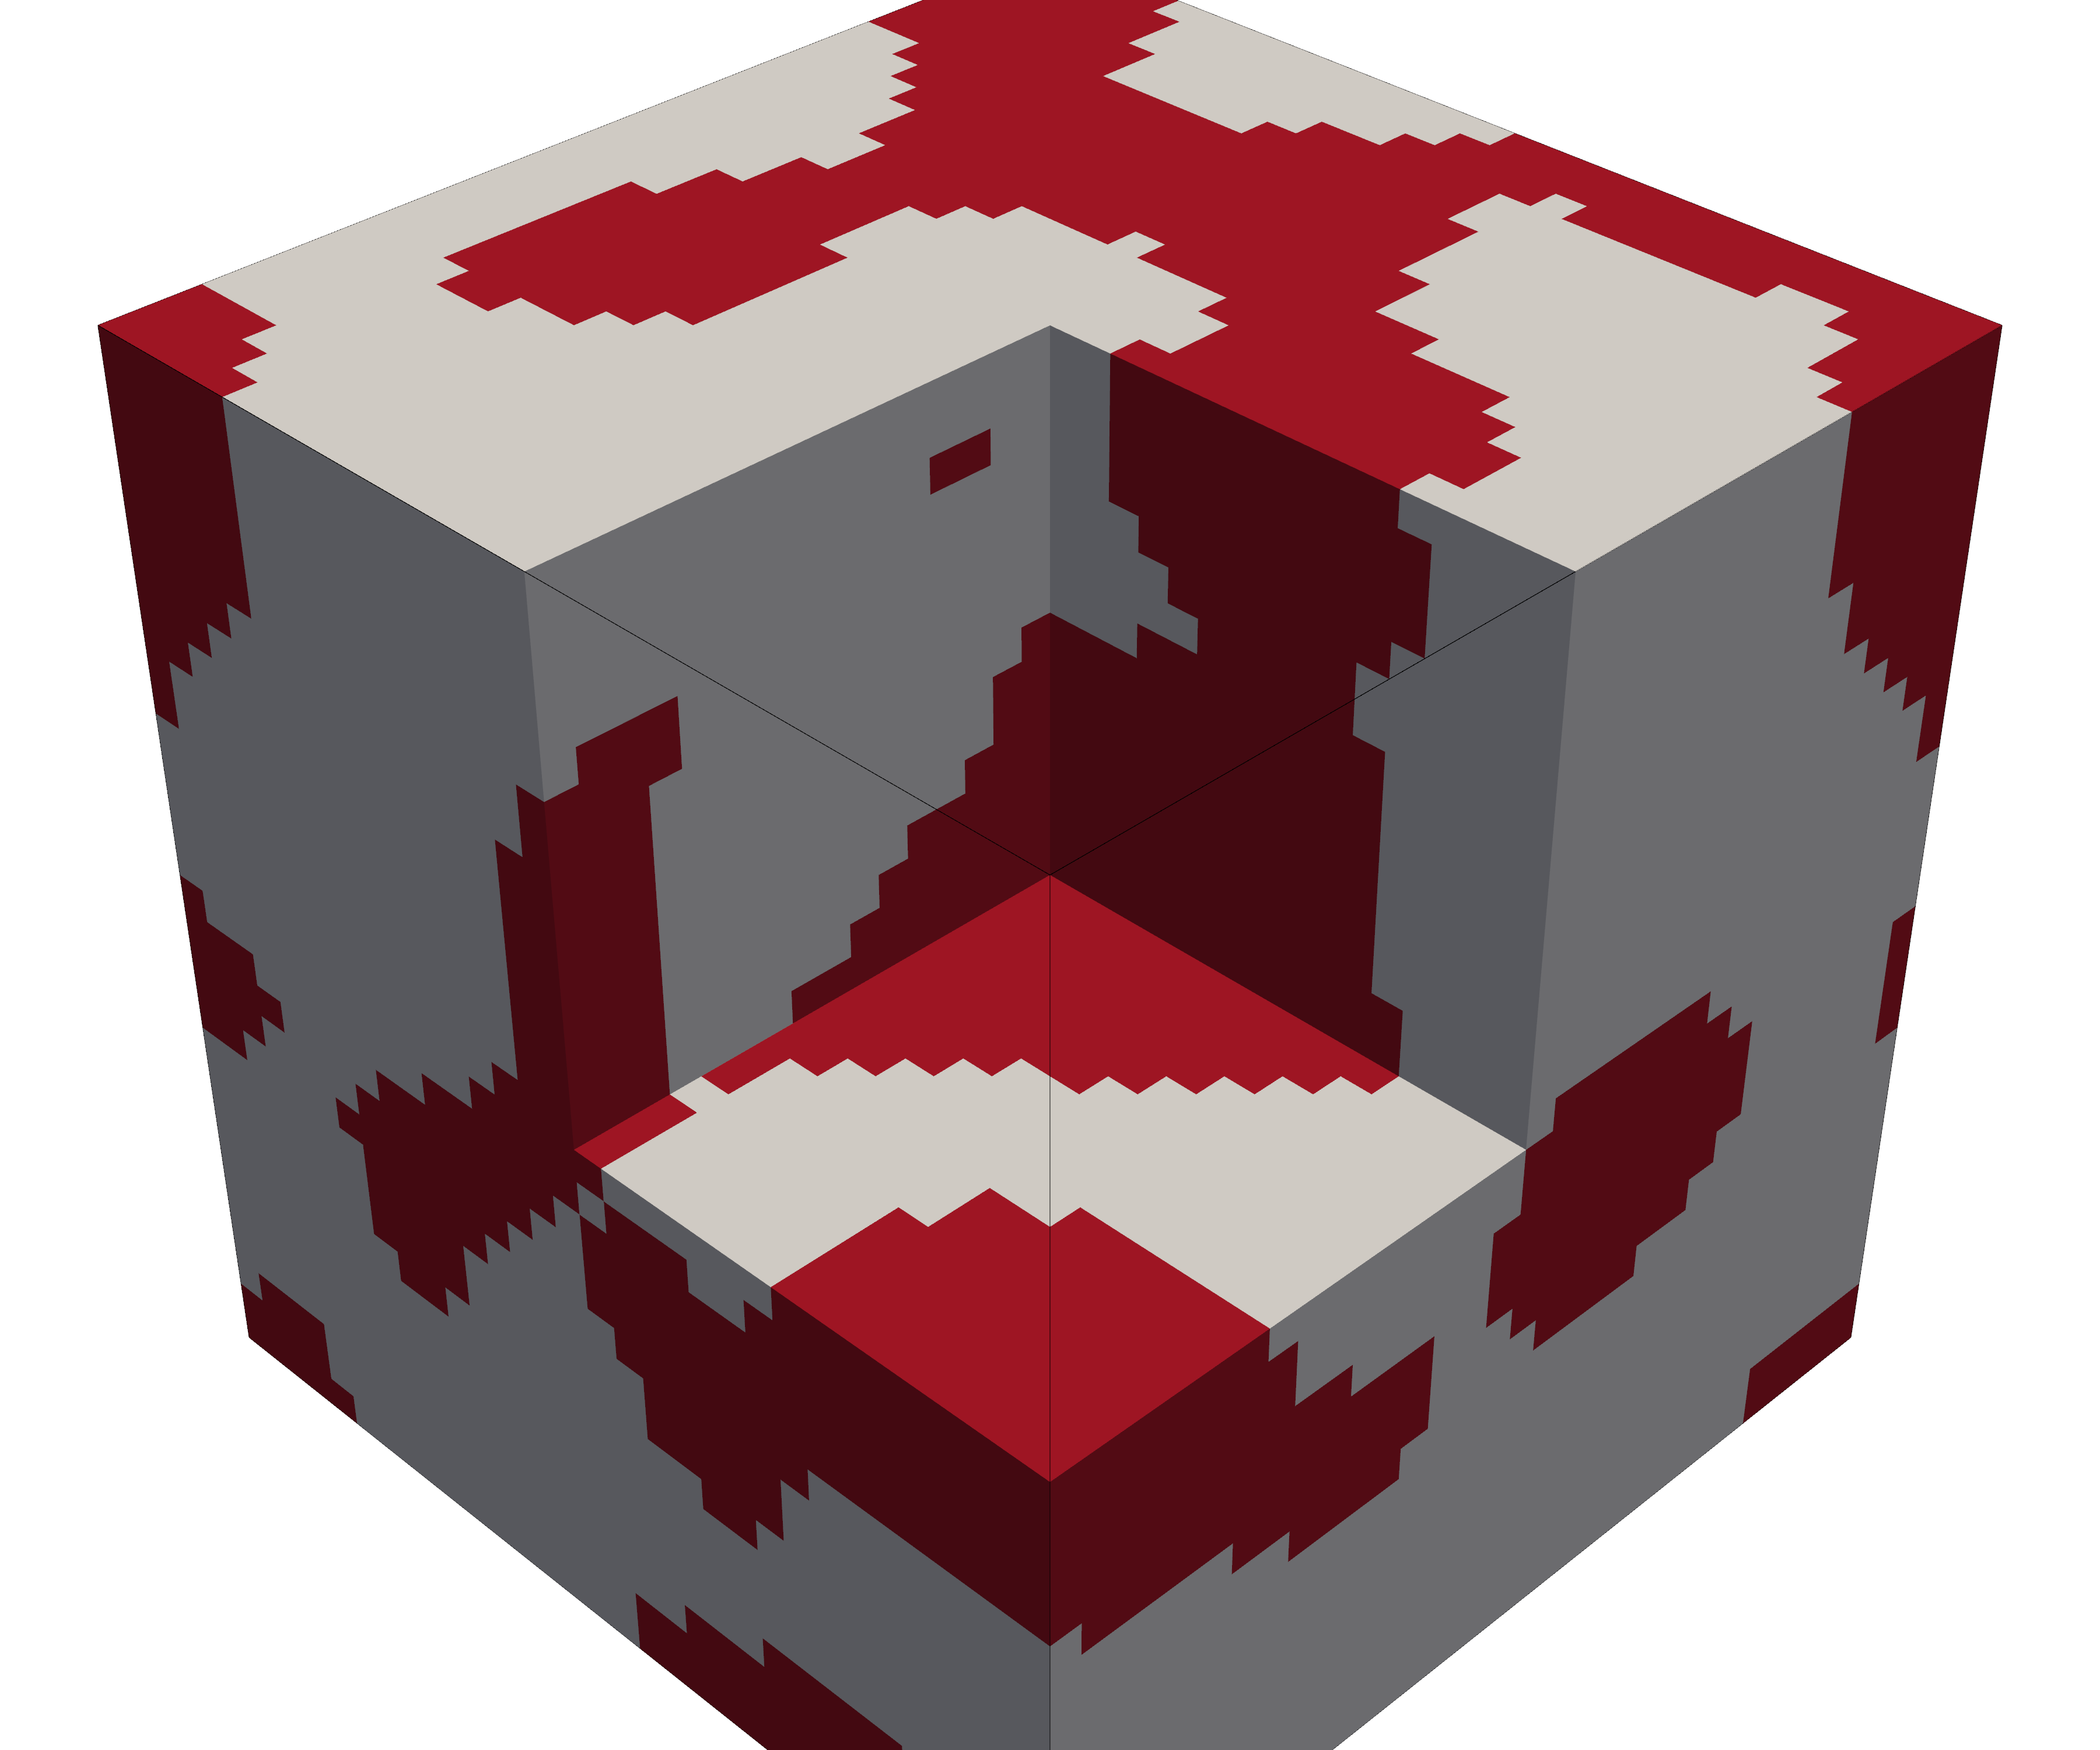
\includegraphics[width=0.55\textwidth]{figures/field_channelized.png}
\caption{The channelized coefficient field on $[0,1]^3$, with a corner octant removed.}
\label{fig:field}
\end{figure}

The measured iteration counts grow with the problem size: at uniform
radius $\rho = 3$ the fitted rates are $N^{0.29}$ for diffusion and
$N^{0.36}$ for elasticity (Figure~\ref{fig:iters_N}).  These radii lie
below the threshold of Corollary~\ref{lem:threshold} at this decay
length, in the regime where Theorem~\ref{prop:precond_conditioning}
guarantees convergence at every radius but permits polynomial growth
of the iteration count (Subsubsection~\ref{rem:consequences}).  The
largest configuration, $2.7$ million unknowns, solves in $45$
iterations.

\begin{figure}[t]
\centering
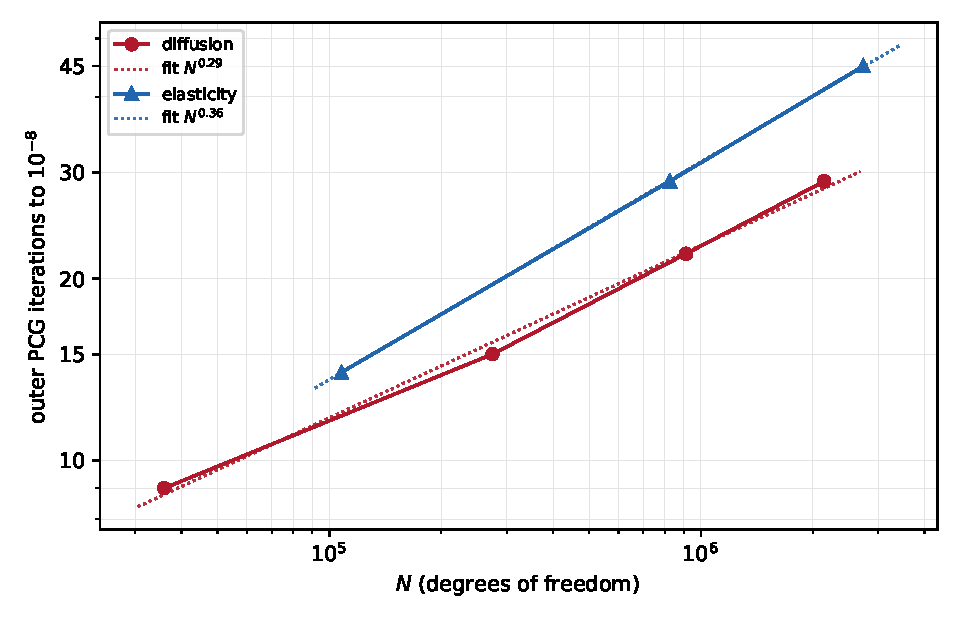
\includegraphics[width=0.8\textwidth]{figures/iters_N.pdf}
\caption{Outer PCG iterations to relative residual $10^{-8}$ as a
function of the problem size, at uniform radius $\rho = 3$, with
fitted power laws.}
\label{fig:iters_N}
\end{figure}
Build time, application time, and both memory footprints grow
linearly in the problem size, at the rates stated in
Proposition~\ref{prop:cost} (Figure~\ref{fig:scaling}); the largest
completed configurations reach several million unknowns on one 80~GB
device (Table~\ref{tab:flagship}).  Growth with the radius at fixed
size is no faster than the model, $\rho^{2d}$ for the build and
$\rho^{d}$ for the application (Table~\ref{tab:cost_vs_rho}).

\begin{figure}[t]
\centering
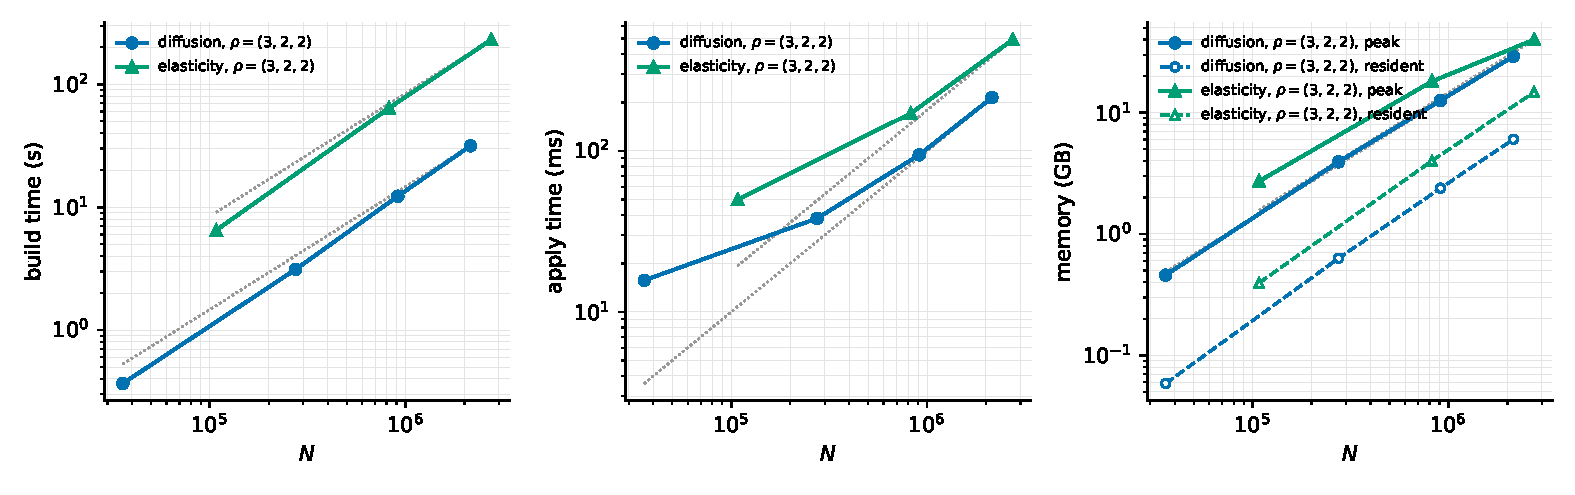
\includegraphics[width=\textwidth]{figures/scaling_ladder.pdf}
\caption{Measured scaling of build time, apply time, and memory with
the problem size at $\rho = (3,2,2)$.}
\label{fig:scaling}
\end{figure}

\begin{table}[t]
\centering
% generated by render_flagship.py from flagship_ladder.json
{\small
\begin{tabular}{llrrrrr}
\toprule
problem & $\rho$ & $N$ & build (s) & solve (s) & iterations & peak (GB) \\
\midrule
diffusion & $(3,2,2)$ & 2\,146\,689 & 31.6 & 11.16 & 41 & 29.1 \\
diffusion & $(4,3,3)$ & 2\,146\,689 & 127.0 & 9.65 & 23 & 40.9 \\
elasticity & $(3,2,2)$ & 2\,738\,019 & 230.9 & 36.15 & 57 & 39.9 \\
elasticity & $(4,3,3)$ & 823\,875 & 459.6 & 6.74 & 19 & 45.0 \\
\bottomrule
\end{tabular}
}
% solve (s): outer PCG wall time; the outer loop runs in Python over on-device
% operations, so iteration counts are the noise-free result and the on-device
% per-application time is apply\_ms in the JSON.

\caption{The largest configurations run on one GPU.}
\label{tab:flagship}
\end{table}

\begin{table}[t]
\centering
% uniform radii by design (the rho-exponent check); category 9
% generated by render_cost_vs_rho.py
{\small
\begin{tabular}{lrrrr}
\toprule
operator & $\rho$ & build (s) & apply (ms) & iterations \\
\midrule
diffusion & 2 & 3.4 & 49 & 46 \\
diffusion & 3 & 27.3 & 109 & 22 \\
diffusion & 4 & 87.3 & 185 & 13 \\
% diffusion: fitted build exponent 5.54 (claimed 6), apply 2.26 (claimed 3)
elasticity & 2 & 52.8 & 217 & 98 \\
elasticity & 3 & 468.5 & 526 & 45 \\
% elasticity: fitted build exponent 6.49 (claimed 6), apply 2.63 (claimed 3)
\bottomrule
\end{tabular}
}

\caption{Build and apply cost as a function of the localization
radius at fixed problem size; three uniform radii, a consistency check
rather than a fit.}
\label{tab:cost_vs_rho}
\end{table}

The inner iteration counts are bounded uniformly in the level and
the problem size, as Corollary~\ref{thm:localized_block_conditioning}
requires: at the finest level, which dominates the cost, the measured
mean does not change across sizes (Table~\ref{tab:inner_iters}).

\begin{table}[t]
\centering
% diffusion only: the elasticity sweep did not record per-level counts
% generated by render_inner_iters.py from sweep_ladder.json
% means over the solve segment at tau = 1e-06
{\small
\begin{tabular}{lrrr}
\toprule
& \multicolumn{3}{c}{inner iterations per block solve} \\
 & level $q$ & level $q-1$ & level $q-2$ \\
\midrule
cr 4 & 24 & 17 & 9 \\
cr 8 & 24 & 18 & 12 \\
cr 12 & 24 & 20 & 12 \\
\bottomrule
\end{tabular}
\par\smallskip
{\footnotesize Means at the working tolerance; the coarsest block is factorized directly and runs no iterations.}
}

\caption{Mean inner CG iterations per block solve at the working
tolerance, diffusion, $\rho = (3,2,2)$.}
\label{tab:inner_iters}
\end{table}

Tightening the memory budget or the batch cap reduces the build
peak by roughly a third before the build time changes by more than a
few percent, and leaves the computed factors unchanged
(Table~\ref{tab:memory}; Subsection~\ref{sec:consequences:build}).

\begin{table}[t]
\centering
% generated by render_memory.py from memory_ladder.json
{\small
\begin{tabular}{lrr}
\toprule
knob & peak (GB) & build (s) \\
\midrule
budget default & 13.4 & 12.2 \\
budget 20\,GB & 12.6 & 12.2 \\
budget 10\,GB & 11.3 & 12.3 \\
budget 5\,GB & 8.5 & 12.0 \\
budget 2.5\,GB & 8.5 & 11.8 \\
\midrule
batch cap 8000 & 8.5 & 11.7 \\
batch cap 4000 & 8.5 & 11.9 \\
batch cap 2000 & 8.5 & 12.4 \\
batch cap 1000 & 8.5 & 13.1 \\
batch cap 500 & 8.5 & 14.1 \\
\bottomrule
\end{tabular}
\par\smallskip
{\footnotesize Resident store 2.39\,GB and 31 outer iterations in every arm.}
}
% peak composition (default arm): peak at post-triple k=3, total 11.25 GB = base 1.21 GB + batch working set 10.04 GB; post-build resident 2.39 GB

\caption{Build peak and build time as functions of the memory budget
and the batch cap, at $cr = 12$.}
\label{tab:memory}
\end{table}

Iterating decouples the achieved accuracy from the build: a single
application of the factorization carries an error that grows with~$N$
at fixed radius, and the preconditioned iteration passes that floor
within its first few steps (Figure~\ref{fig:decoupling}).

\begin{figure}[t]
\centering
% floor definition (scale-optimal) pending the author's ruling and the
% c* normalization trace
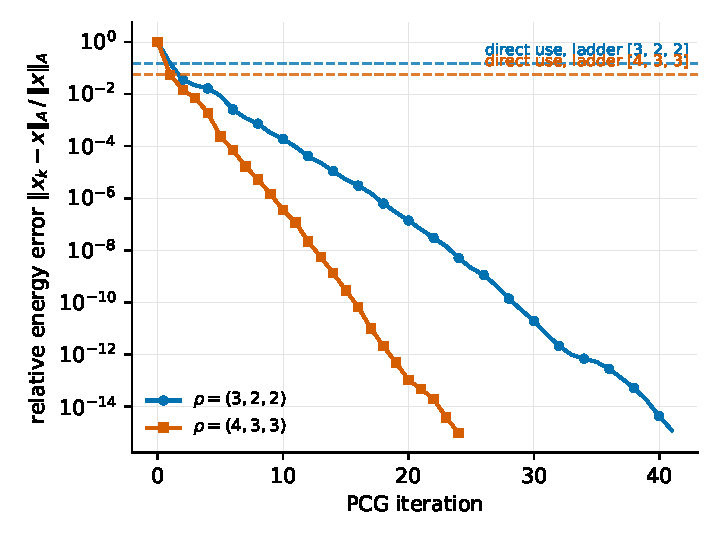
\includegraphics[width=0.8\textwidth]{figures/decoupling_ladder.pdf}
\caption{Error as a function of the iteration count for a single build,
with the direct-use error floor of the same factorization, defined as
the scale-optimal single application.}
\label{fig:decoupling}
\end{figure}

The outer iteration is insensitive to the inner tolerance: across
five orders of magnitude the count moves by at most two iterations and
the achieved error stays at the reference level
(Table~\ref{tab:inner_tol}); this is the measurement to which
Remark~\ref{rem:inexact} defers the inner-residual effect.

\begin{table}[t]
\centering
% generated by render_inner_tol.py from sweep_ladder.json
% tau* = 1e-06 (tau* = loosest tau such that, for EVERY cr in the sweep: the outer sol...)
{\small
\begin{tabular}{lrrrrrrrr}
\toprule
& \multicolumn{8}{c}{inner tolerance $\tau$} \\
outer iterations & $10^{-1}$ & $10^{-2}$ & $10^{-3}$ & $10^{-4}$ & $10^{-5}$ & $\mathbf{10^{-6}}$ & $10^{-7}$ & $10^{-8}$ \\
\midrule
cr 4 & 13 & 11 & 10 & 10 & 10 & 10 & 10 & 10 \\
cr 8 & 28 & 22 & 22 & 22 & 20 & 20 & 20 & 20 \\
cr 12 & 43 & 36 & 33 & 33 & 31 & 31 & 31 & 31 \\
\bottomrule
\end{tabular}
\par\smallskip
{\footnotesize Achieved energy errors relative to the $10^{-12}$ reference are at most $10^{-10}$ in every cell.}
}

\caption{Outer PCG iterations as a function of the inner tolerance;
the tolerance used in all other experiments is fixed from this table.}
\label{tab:inner_tol}
\end{table}


\subsection{Comparison with multigrid baselines}
\begin{itemize}
  \item Claim substantiated: the introduction's comparison with algebraic
    multigrid on high-contrast fields.
    \item Design: GPU algebraic multigrid baselines (GAMG, BoomerAMG) on
    the same fields, same hardware, same tolerances: setup time, solve
    time, iterations, memory; CPU pyAMG rows report iterations and
    convergence only; prior OAW implementations enter as cited
    published numbers, not reruns.
  \item Reading: iteration counts on par with BoomerAMG, and robustness
    exceeding GAMG and pyAMG, which fail on the large elasticity
    systems; setup and solve wall-clock favor the production AMG codes,
    conceded plainly; the amortization argument compares the
    preconditioner with the direct use of the same factorization
    (Section~\ref{sec:main_bounds}), not with multigrid.
\end{itemize}
% Baseline environments: GAMG-GPU; BoomerAMG via the from-source
% pdes-hypre-gpu environment (conda hypre is CPU-only).
\begin{table}[t]
\centering
% PLACEHOLDER render: uniform-radius gamblet rows (2026-11-02); ladder
% rerun + pyAMG rows pending.
% generated by render_baselines.py
{\small
\begin{tabular}{lrrrrrr}
\toprule
system & $N$ & gamblet, $\rho=(3,2,2)$ & GAMG & BoomerAMG & pyAMG-SA & pyAMG-RS \\
\midrule
diffusion cr\,4 & 35\,937 & 10 & 12 & 14 & 9 & 8 \\
elasticity cr\,4 & 107\,811 & 16 & 7$^{b}$ & 35 & 58 & 61 \\
diffusion cr\,8 & 274\,625 & 20 & 14 & 16 & 10 & 14 \\
elasticity cr\,8 & 823\,875 & 35 & 38 & 38 & 116 & --$^{a}$ \\
diffusion cr\,12 & 912\,673 & 31 & 15 & 17 & 12 & 20 \\
diffusion cr\,16 & 2\,146\,689 & 41 & 16 & 19 & 11 & 25 \\
elasticity cr\,12 & 2\,738\,019 & 57 & --$^{a}$ & 39 & 173 & --$^{a}$ \\
elasticity cr\,16 & 6\,440\,067 & -- & --$^{a}$ & 43 & 200$^{c}$ & --$^{a}$ \\
\bottomrule
\end{tabular}
\par\smallskip
{\footnotesize Outer iterations to relative residual $10^{-8}$; setup and solve times are reported in the text.  $^{a}$setup failure; $^{b}$converged in the preconditioned norm only; $^{c}$not converged in 200 iterations.}
}

\caption{Comparison with GPU algebraic multigrid baselines and published
OAW implementations.}
\label{tab:baselines}
\end{table}

\subsection{Equivalence classes}
\label{sec:exp:classes}

Theorem~\ref{thm:row_equality} licenses solving and storing one
representative per translation class.  Table~\ref{tab:classes} reports
the effect on the two structured fields: the fraction of distinct
rows, from the measured class counts, and the measured reduction in
patch-solve and total build time.  The fraction falls with the problem size, since the interior
classes are fixed by the field's period while the boundary classes
grow as a surface.  The solve-time reduction grows accordingly; at the
smallest size the classification overhead exceeds the saving.  Under the stencil format the value table holds
one row per class, so within each level the stored values fall by that
level's class fraction.  A field without local translation symmetry
reduces to singleton classes and gains nothing.

\begin{table}[t]
\centering
% storage column switches to measured bytes when category 18 lands
% generated by render_class_table.py from dedup_time_ladder.json
% distinct-row fraction from measured class counts; speedups
% relative to the identity class map (dedup off)
{\small
\begin{tabular}{llrrr}
\toprule
field & size & distinct rows & patch solve & build \\
\midrule
checkerboard & cr 4 & 40.6\% & $1.1\times$ & $1.0\times$ \\
 & cr 8 & 12.4\% & $2.8\times$ & $1.6\times$ \\
 & cr 12 & 6.2\% & $5.7\times$ & $1.9\times$ \\
\midrule
periodic sandwich & cr 4 & 38.7\% & $1.0\times$ & $0.4\times$ \\
 & cr 8 & 9.0\% & $2.7\times$ & $1.5\times$ \\
 & cr 12 & 3.3\% & $6.2\times$ & $1.9\times$ \\
\bottomrule
\end{tabular}
\par\smallskip
{\footnotesize Distinct rows: solved and stored classes as a fraction of all rows, from the measured class counts.  Speedups: time with the identity class map over time with the class map.}
}

\caption{Effect of the class map on the structured fields: distinct
rows as a fraction of all rows, and measured speedups relative to the
identity class map.}
\label{tab:classes}
\end{table}

\subsection{Time-dependent problems}
\begin{itemize}
    \item Claim substantiated: Theorem~\ref{thm:perturbed_system} and the
    introduction's time-stepping claim: a hierarchy built once
    preconditions every step of a variable-step scheme.
  \item Design: implicit time stepping of a parabolic problem on the
    canonical field; the hierarchy is built for the operator at one
    reference step size and reused unchanged while the step size varies
    over several orders of magnitude; outer iterations per linear solve
    recorded, no rebuilds.
    \item Reading: iterations as a function of the ratio of the step size
    to the reference, with both wings of the measured V inside the
    $\sqrt{\max\{\tau/\tau_0,\,\tau_0/\tau\}}$ envelope of
    Theorem~\ref{thm:perturbed_system}; the cost of the avoided
    per-step rebuilds is read from the build column of the scaling
    subsection.
\end{itemize}
\begin{figure}[t]
\centering
% PLACEHOLDER render: uniform rho=3 (2026-11-02); ladder rerun pending.
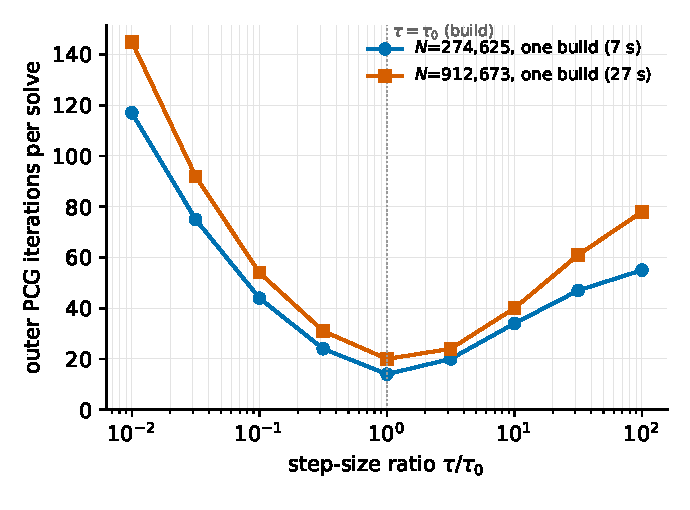
\includegraphics[width=0.8\textwidth]{figures/timestep.pdf}
\caption{Iteration counts across time steps for a hierarchy built once
at a reference step size.}
\label{fig:timestep}
\end{figure}

\section{Conclusions}
\label{sec:conclusions}
% BP JOB: limitations and open questions; open questions here and nowhere
%     else
We have presented a construction and convergence rate bound for for a conjugate-gradient preconditioner based on operato adapted wavelets, with quasi-optimal convergence and demonstrated scalability to large three-dimensional problems beyond the capabilities of the original direct-solver algorithm. There are a number of limitations that may be worth pursuing in future work. Firstly, in our analysis the choice of measurement hierarchy is fixed a-priori, but the complexity of the algorithm does not change substantially if the coarse subspaces are selected dynamically based on the operator, which is closer to standard multigrid practice and may lead to superior convergence properties. The analysis is also restricted entirely to SPD systems, and a generalization to non-symmetric systems with distinct test and trial spaces (analogous to \cite{HauckPeterseim2021}) would close this gap. Also, the present paper is restricted to unstructured meshes and first order finite element trial spaces, and generalizing to unstructured meshes and higher-order elements would be indispensable to a production-quality implementation. Similarly, modifying the algorithm to work across multiple devices or optimizing the memory access mechanics, is a nontrivial endeavor crucial to practical adoption fo the method that we have not pursued.

\section*{Acknowledgments}
% TODO: carried from main_abridged.tex at harvest.

\section*{Code and data availability}
% TODO: carried from main_abridged.tex at harvest.
$\cdots$\\
% Appendices extracted to main_curr_v2_appendices.tex (2026-10-24) for
% modularity and paper-proper page counts; re-enable by uncommenting.
% \appendix

TODO: Clean up appendix, currently it's a parking spot for deprecated prose
\section{The OAW factorization from first principles}
\label{app:oaw}

This appendix derives the coarse spaces and the multiresolution basis by
duality, the recursive construction, and the direct use of the
factorization, complementing the definitions of
Section~\ref{sec:background}.

\subsection{Coarse spaces and duality}
\label{app:oaw:duality}

% The coarse spaces
Each level of measurements induces a coarse space of trial functions.
Fix~$k$ and let
\[
  \mathcal{N}^{(k)} := \bigcap_{j=1}^{n_k} \ker \mu^{(k)}_j
  \;\subset\; \mathcal{V}^{(q)}
\]
be the common kernel of the level-$k$ functionals, the subspace of trial
functions invisible to the level-$k$ measurements.  We identify the dual space of
$\mathcal{V}^{(k)*}$ with a subspace of
$\mathcal{V}^{(q)}$  using the orthogonal complement in the energy product induced by $a$,
\[
  \mathcal{V}^{(k)} := \bigl(\mathcal{N}^{(k)}\bigr)^{\perp_a}
  = \bigl\{ v \in \mathcal{V}^{(q)} : a(v,w) = 0
    \text{ for all } w \in \mathcal{N}^{(k)} \bigr\},
\]
Since the functionals are linearly independent, this space has dimension~$n_k$. The
nesting~\eqref{eq:measurement_nesting} implies decreasing kernels, $\mathcal{N}^{(k)} \supseteq \mathcal{N}^{(k+1)}$, so the
coarse spaces are nested: $\mathcal{V}^{(k)} \subset \mathcal{V}^{(k+1)}$
for $1 \leq k < q$.

The level-$k$ \emph{detail space} is defined as
\[
  \mathcal{W}^{(k)} := \mathcal{V}^{(k+1)} \cap \mathcal{N}^{(k)} .
\]
It is $a$-orthogonal to $\mathcal{V}^{(k)}$ by construction, and every
$y \in \mathcal{V}^{(k+1)}$ splits under $\mathcal{V}^{(q)} =
\mathcal{V}^{(k)} \oplus_a \mathcal{N}^{(k)}$ as $y = v + w$ with $v \in
\mathcal{V}^{(k)}$ and $w = y - v \in \mathcal{W}^{(k)}$, so
\begin{equation}
  \mathcal{V}^{(k+1)} = \mathcal{V}^{(k)} \oplus_a \mathcal{W}^{(k)},
  \qquad
  \mathcal{V}^{(q)} = \mathcal{V}^{(1)} \oplus_a \mathcal{W}^{(1)}
  \oplus_a \cdots \oplus_a \mathcal{W}^{(q-1)} .
\end{equation}

% The bases
The level-$k$ OAW basis is the basis of $\mathcal{V}^{(k)}$ dual to its
measurements:
\begin{equation}\label{eq:dual_basis}
  \psi^{(k)}_i \in \mathcal{V}^{(k)},
  \qquad \mu^{(k)}_j\bigl(\psi^{(k)}_i\bigr) = \delta_{ij},
  \qquad 1 \leq i, j \leq n_k .
\end{equation}
It exists and is unique: a function in $\mathcal{V}^{(k)}$ annihilated by
every level-$k$ measurement lies in $\mathcal{V}^{(k)} \cap
\mathcal{N}^{(k)} = \{0\}$, so the measurement map $v \mapsto
(\mu^{(k)}_j(v))_j$ is injective on $\mathcal{V}^{(k)}$, and is bijective
since the dimensions agree.

The function $\psi^{(k)}_i$ is also the minimum-energy trial function with
its measurements: over the affine constraint set
\begin{equation}
  \mathcal{A}^{(k)}_i
  := \{v \in \mathcal{V}^{(q)} : \mu^{(k)}_j(v) = \delta_{ij},\;
       1 \leq j \leq n_k\}
\end{equation}
it satisfies
\begin{equation}
    \psi^{(k)}_i = \operatorname{argmin}_{f \in \mathcal{A}^{(k)}_i} \lVert f\rVert_a \, ,
\end{equation}
since every $f \in \mathcal{A}^{(k)}_i$ differs from $\psi^{(k)}_i$ by an
element of $\mathcal{N}^{(k)}$, so that $\lVert f \rVert_a^2 = \lVert
\psi^{(k)}_i \rVert_a^2 + \lVert f - \psi^{(k)}_i \rVert_a^2$.

\begin{comment}
Membership in $\mathcal{V}^{(k)} = (\mathcal{N}^{(k)})^{\perp_a}$ states
that the functional $a(\psi^{(k)}_i, \cdot) \in (\mathcal{V}^{(q)})^*$
annihilates~$\mathcal{N}^{(k)}$.  The functionals annihilating
$\mathcal{N}^{(k)}$ form a space of dimension $n_k$ containing
$\mathcal{V}^{(k)*}$, so the two coincide, and there are coefficients
$\lambda^{(k)}_{i\ell}$ with
\begin{equation}\label{eq:gamblet_basis}
a(\psi^{(k)}_i, v)= \sum_{\ell=1}^{n_k}\lambda^{(k)}_{i\ell}\,\mu^{(k)}_\ell(v)
\quad \forall v \in \mathcal{V}^{(q)},
\qquad
\mu^{(k)}_j(\psi^{(k)}_i) = \delta_{ij}.
\end{equation}
In the minimization problem
~\eqref{eq:psi_k_def}, the $\lambda^{(k)}_{i\ell}$ are the Lagrange
multipliers associated with the measurement constraints.
\end{comment}

The detail space $\mathcal{W}^{(k)}$ has dimension $d_k = n_{k+1} - n_k$
by~\eqref{eq:scale_decomposition}. The functions $\chi^{(k)}_i$, $1 \leq i \leq d_k$
\begin{equation}
  \chi^{(k)}_j = \sum_{\ell=1}^{n_{k+1}} D^{(k)}_{j\ell}\,\psi^{(k+1)}_\ell,
  \qquad 1 \leq j \leq d_k,
\end{equation}
form a basis for $\mathcal{W}^{(k)}$. To see this, we need only recall that the $\psi^{(k+1)}_{\ell}$ are linearly independent, that $D^{(k)}$ has full row rank, and count dimensions.

\begin{theorem}[Exponential energy decay
{\cite[Thm.~15.41, (15.127)]{Owhadi_Scovel_2019}}]\label{thm:energy_decay}
  Let $B_r(x^{(k)}_i)$ denote the ball of radius $r h_k$ about the
  node~$x^{(k)}_i$ of $\psi^{(k)}_i$.  Then
  \begin{equation}\label{eq:energy_decay}
    \|\psi^{(k)}_i\|_{a,\, B_r(x^{(k)}_i)^c}^2
    \;\leq\;
    e^{1 - r/\ell}\,\|\psi^{(k)}_i\|_a^2 ,
  \end{equation}
  where the decay length~$\ell$, measured in level-$k$ mesh widths, is
  independent of $N$, of the level, and of the discretization; the physical
  decay length is $\ell h_k$.
\end{theorem}

\subsection{The exact recursion}
\label{sec:background:oaw}

Problem~\eqref{eq:gamblet_basis} is posed in~$\mathcal{V}^{(q)}$: computed
directly, the basis at level~$k$ requires $n_k$ solves in a space of
dimension~$n_q$, which gives a total cost superlinear in~$n_q$, the
precomputation cost of LOD
methods~\cite{hauck2022multiresolutionlocalizedorthogonaldecomposition}.
We now show how the nesting of the coarse spaces circumvents this cost:
each level-$k$ basis function is a linear combination of the level-$(k+1)$
basis functions, so the problems characterizing the basis functions at
level~$k$ may be posed in the coordinates of the adjacent level~$k+1$,
rather than the full trial space.  Explicitly, define the
\emph{refinement matrix} $R^{(k)} \in \mathbb{R}^{n_k \times n_{k+1}}$ by
\begin{equation}\label{eq:prolongation}
  \psi^{(k)}_i = \sum_{\ell=1}^{n_{k+1}} R^{(k)}_{i\ell}\,\psi^{(k+1)}_\ell,
  \qquad 1 \leq i \leq n_k .
\end{equation}
Evidently, it suffices to compute the coefficients $R^{(k)}_{i\ell}$, or,
equivalently, the rows of~$R^{(k)}$; we now characterize these rows in
terms of quantities available at level~$k+1$.  Applying $\mu^{(k)}_j$
to~\eqref{eq:prolongation} and using~\eqref{eq:nesting_maps} with the
level-$(k+1)$ biorthogonality~\eqref{eq:dual_basis} gives the
\emph{measurement constraint}
\begin{equation}\label{eq:measurement_constraint}
  C^{(k)}\,R^{(k)\top} = I_{n_k} ,
\end{equation}
so $R^{(k)\top}$ is a right inverse of $C^{(k)}$.  Since each $\psi^{(k)}_i$
minimizes energy subject to that constraint~\eqref{eq:psi_k_def}, the $i$-th
row of~$R^{(k)}$ solves
\begin{equation}\label{eq:R_minimization}
  R^{(k)\top} e_i
  = \operatorname*{argmin}_{r \in \mathbb{R}^{n_{k+1}}} r^\top A^{(k+1)} r
  \quad \text{subject to} \quad C^{(k)}\,r = e_i ,
\end{equation}
where $A^{(k+1)}_{ij} = a(\psi^{(k+1)}_i, \psi^{(k+1)}_j)$.  Thus $R^{(k)\top}$
is the $A^{(k+1)}$-optimal right inverse of~$C^{(k)}$.

The KKT conditions for~\eqref{eq:R_minimization} read
\begin{equation}\label{eq:kkt}
  A^{(k+1)}\,r + C^{(k)\top}\lambda = 0,
  \qquad C^{(k)}\,r = e_i .
\end{equation}
Any feasible $r$ may be written $r = C^{(k)\dagger\top} e_i + D^{(k)\top} z$
with $C^{(k)\dagger\top}$ a right inverse of $C^{(k)}$ and the second term in
$\ker C^{(k)} = \operatorname{range}(D^{(k)\top})$.  Substituting and
left-multiplying by~$D^{(k)}$ eliminates $C^{(k)\top}\lambda$, leaving
\begin{equation}\label{eq:z_solve}
  B^{(k+1)}\,z_i = -D^{(k)}\,A^{(k+1)}\,C^{(k)\dagger\top} e_i ,
  \qquad
  B^{(k+1)} := D^{(k)}\,A^{(k+1)}\,D^{(k)\top},
\end{equation}
where $B^{(k+1)}$ is the restriction of $A^{(k+1)}$ to $\ker C^{(k)}$, and is
the same matrix as the $(k+1)$-th diagonal block of~\eqref{eq:block_diagonal}.
Collecting the solutions $z_i$ as the rows of~$Z^{(k)}$,
\begin{equation}\label{eq:R_assembly}
  R^{(k)} = C^{(k)\dagger} + Z^{(k)}\,D^{(k)} ,
\end{equation}
and the coarsened stiffness
\begin{equation}\label{eq:coarsened_stiffness}
  A^{(k)} = R^{(k)}\,A^{(k+1)}\,R^{(k)\top}
\end{equation}
is the input for level $k-1$.  The recursion runs from $A^{(q)} = K$ down to
$A^{(1)}$.  Note that $R^{(k)}$, and therefore $A^{(k)}$, is independent of
the choice of $C^{(k)\dagger}$ (Lemma~\ref{lem:cdagger_independence}).

The full recursive construction is given in
Algorithm~\ref{alg:exact_build}.  The matrices
$\Psi^{(k)} \in \mathbb{R}^{n_k \times n_q}$ and $X^{(k)} \in
\mathbb{R}^{d_k \times n_q}$ hold the coefficients of the level-$k$ basis
functions $\psi^{(k)}_i$ and $\chi^{(k)}_j$ in the fine-mesh basis, and
satisfy $\Psi^{(k)} = R^{(k)}\Psi^{(k+1)}$ and $X^{(k)} =
D^{(k)}\Psi^{(k+1)}$.  They are the blocks of the change of basis
of~\eqref{eq:combined_basis}: since $n_1 + d_1 + \cdots + d_{q-1} = n_q$,
\begin{equation}\label{eq:Psi_blocks}
  \Phi^\top =
  \begin{bmatrix}
    \Psi^{(1)} \\ X^{(1)} \\ \vdots \\ X^{(q-1)}
  \end{bmatrix}.
\end{equation}

\begin{algorithm}[t]
\caption{Exact OAW construction}
\label{alg:exact_build}
\textbf{Input:} $A^{(q)} = K$, $\Psi^{(q)} = I$; nesting maps
$\{C^{(k)}\}_{k=1}^{q-1}$; detail maps $\{D^{(k)}\}_{k=1}^{q-1}$\\[4pt]
\textbf{for} $k = q-1, q-2, \ldots, 1$ \textbf{do}
\begin{enumerate}
  \item[1.] Compute $C^{(k)\dagger}$ with $C^{(k)}\,C^{(k)\dagger\top} = I_{n_k}$.
  \item[2.] Form $B^{(k+1)} \gets D^{(k)}\,A^{(k+1)}\,D^{(k)\top}$.
  \item[3.] \textbf{for} $i = 1, \ldots, n_k$ \textbf{do} solve
    $B^{(k+1)}\, z_i = -D^{(k)}\,A^{(k+1)}\,C^{(k)\dagger\top} e_i$.
  \item[4.] Assemble $R^{(k)} \gets C^{(k)\dagger} + Z^{(k)}\,D^{(k)}$.
  \item[5.] Coarsen $A^{(k)} \gets R^{(k)}\,A^{(k+1)}\,R^{(k)\top}$.
  \item[6.] Accumulate $X^{(k)} \gets D^{(k)}\,\Psi^{(k+1)}$ and
    $\Psi^{(k)} \gets R^{(k)}\,\Psi^{(k+1)}$.
\end{enumerate}
\textbf{end for.}  \textbf{Output:} $\{\Psi^{(k)}\}$, $\{X^{(k)}\}$,
$\{B^{(k)}\}$, $\{A^{(k)}\}$.
\end{algorithm}

\subsection{The direct approximate inverse}
\label{sec:background:apply}

Replacing the exact factors in~\eqref{eq:exact_inverse_formula} by the
localized ones gives an approximate direct solver: the approximate solution
of $Ku = g$ is
\begin{equation}\label{eq:localized_inverse}
  \hat{u}_\rho \;:=\;
  \Phi_\rho \operatorname{diag}\bigl( B^{(k)\,-1}_\rho \bigr)\,
  \Phi_\rho^\top\, g ,
\end{equation}
computed by a projection, one independent block solve per level, and a
recombination.  The procedure, in terms of the stored factors of
Algorithm~\ref{alg:recursive_build}, is given as
Algorithm~\ref{alg:direct_solve}.  Once the factors are built, each
right-hand side costs one projection, $q$ block solves, and one
recombination, in total $\mathcal{O}(N\rho^{d})$ operations, proportional
to the number of stored entries of the factors~\cite{owhadi2017}.
% TODO: verify the O(N rho^d) apply accounting against owhadi2017 (stored
% block factors vs iterative block solves); the full accounting is
% Section 4's.

The localized factors and the accumulated blocks $\Psi^{(1)}$,
$\{X^{(k)}\}$ are produced by Algorithm~\ref{alg:recursive_build},
the standard form of the literature (cf.~\cite{budni2019}).

\begin{algorithm}[t]
\caption{Localized OAW construction (cf.~\cite{budni2019})}
\label{alg:recursive_build}
\textbf{Input:} $A^{(q)} = K$, $\Psi^{(q)} = I$; nesting maps
$\{C^{(k)}\}_{k=1}^{q-1}$; detail maps $\{D^{(k)}\}_{k=1}^{q-1}$; radius
$\rho$\\[4pt]
\textbf{for} $k = q-1, q-2, \ldots, 1$ \textbf{do}
\begin{enumerate}
  \item[1.] Compute a sparse $C^{(k)\dagger}$ with
    $C^{(k)}\,C^{(k)\dagger\top} = I_{n_k}$.
  \item[2.] Form $B^{(k+1)} \gets D^{(k)}\,A^{(k+1)}\,D^{(k)\top}$.
  \item[3.] \textbf{for} $i = 1, \ldots, n_k$ \textbf{do}
  \begin{enumerate}
    \item[(a)] Identify the patch $\mathcal{P}_i$ of detail indices whose
      detail functions are supported in~$S^{(k)}_i$.
    \item[(b)] Solve $[B^{(k+1)}]_{\mathcal{P}_i}\, z_i =
      -[D^{(k)}\,A^{(k+1)}\,C^{(k)\dagger\top} e_i]_{\mathcal{P}_i}$.
  \end{enumerate}
  \item[4.] Assemble $R^{(k)} \gets C^{(k)\dagger} + Z^{(k)}\,D^{(k)}$;
    threshold small entries.
  \item[5.] Coarsen $A^{(k)} \gets R^{(k)}\,A^{(k+1)}\,R^{(k)\top}$;
    threshold small entries.
  \item[6.] Accumulate $X^{(k)} \gets D^{(k)}\,\Psi^{(k+1)}$ and
    $\Psi^{(k)} \gets R^{(k)}\,\Psi^{(k+1)}$.
\end{enumerate}
\textbf{end for.}  \textbf{Output:} $\{\Psi^{(k)}\}$, $\{X^{(k)}\}$,
$\{B^{(k)}\}$, $\{A^{(k)}\}$.
\end{algorithm}

\begin{algorithm}[t]
\caption{Direct solve with the localized factorization}
\label{alg:direct_solve}
\textbf{Input:} right-hand side $g$; factors $\Psi^{(1)}$,
$\{X^{(k)}\}_{k=1}^{q-1}$, $A^{(1)}$, $\{B^{(k)}\}_{k=2}^{q}$ from
Algorithm~\ref{alg:recursive_build}\\[4pt]
\begin{enumerate}
  \item[1.] Project: $w^{(1)} \gets \Psi^{(1)} g$ and
    $w^{(k+1)} \gets X^{(k)} g$ for $1 \leq k \leq q-1$.
  \item[2.] Solve $A^{(1)} c^{(1)} = w^{(1)}$ and
    $B^{(k+1)}\, c^{(k+1)} = w^{(k+1)}$ for $1 \leq k \leq q-1$.
  \item[3.] Recombine: $\hat{u}_\rho \gets \Psi^{(1)\top} c^{(1)}
    + \sum_{k=1}^{q-1} X^{(k)\top} c^{(k+1)}$.
\end{enumerate}
\textbf{Output:} $\hat{u}_\rho$.
\end{algorithm}


\section{Deferred proofs and technical remarks}
\label{app:proofs}

\begin{lemma}[Independence of the right inverse]\label{lem:cdagger_independence}
The matrix $R^{(k)}$ assembled in~\eqref{eq:R_assembly} from the solutions
of~\eqref{eq:z_solve}, and with it the coarsened
stiffness~\eqref{eq:coarsened_stiffness}, is the same for every
$C^{(k)\dagger}$ with $C^{(k)} C^{(k)\dagger\top} = I_{n_k}$.
\end{lemma}

\begin{proof}
Within this proof fix the level and drop its superscripts, writing $C$,
$D$, $A$, $B = DAD^\top$; $A$ is SPD and $D$ has
full row rank, so $B$ is SPD.  Let $C_1^{\dagger}$
and $C_2^{\dagger}$ satisfy $C C_1^{\dagger\top} = C C_2^{\dagger\top} = I$,
and fix a row index~$i$.  The two candidate rows are
\[
  r^{(j)} = C_j^{\dagger\top} e_i + D^\top z^{(j)},
  \qquad
  B z^{(j)} = -D A\, C_j^{\dagger\top} e_i,
  \qquad j = 1, 2 .
\]
The difference of the baselines is annihilated by $C$ and therefore lies in
$\ker C = \operatorname{range}(D^\top)$:
\[
  \bigl(C_1^{\dagger\top} - C_2^{\dagger\top}\bigr) e_i = D^\top w
  \quad \text{for some } w .
\]
Subtracting the two linear systems and substituting,
\[
  B\bigl(z^{(1)} - z^{(2)}\bigr)
  = -D A \bigl(C_1^{\dagger\top} - C_2^{\dagger\top}\bigr) e_i
  = -D A D^\top w = -B w ,
\]
so $z^{(1)} - z^{(2)} = -w$ by invertibility of $B$, and
\[
  r^{(1)} - r^{(2)}
  = D^\top w + D^\top\bigl(z^{(1)} - z^{(2)}\bigr) = 0 .
\]
The rows coincide, so the assembled matrices coincide, and with them
$A^{(k)} = R^{(k)} A^{(k+1)} R^{(k)\top}$.
\end{proof}


\begin{lemma}[Linear independence of the localized family]\label{lem:localized_independence}
The functions $\varphi_{\rho,i}$, $1 \leq i \leq n_q$, of
Section~\ref{sec:background} are linearly independent.
\end{lemma}

\begin{proof}
Let $\sum_i c_i \varphi_{\rho,i} = 0$ and group the coefficients by
level, $c = (c^{(1)}, t^{(1)}, \ldots, t^{(q-1)})$, with $c^{(1)}$ the
coefficients of the $\psi^{(1)}_{\rho,i}$ and $t^{(k)}$ those of the
$\chi^{(k)}_{\rho,m}$.  For $j \geq k$, the
nesting~\eqref{eq:nesting_maps} and the own-level
data~\eqref{eq:own_level_data} give
$\mu^{(k)}_i(\chi^{(j)}_{\rho,m})
 = (C^{(k)} \cdots C^{(j)} D^{(j)\top})_{im} = 0$
by~\eqref{eq:kernel_D}.  Applying the level-1 functionals to the
vanishing combination therefore yields $c^{(1)} = 0$.  Assume
$c^{(1)} = 0$ and $t^{(1)} = \cdots = t^{(k-1)} = 0$.  Applying the
level-$(k{+}1)$ functionals annihilates every term of level $j > k$ and
evaluates the level-$k$ term through
$\mu^{(k+1)}_i(\chi^{(k)}_{\rho,m}) = D^{(k)}_{mi}$, so
$D^{(k)\top} t^{(k)} = 0$ and $t^{(k)} = 0$ by the rank condition
in~\eqref{eq:kernel_D}.  Induction over the levels gives $c = 0$.
\end{proof}

\begin{lemma}[Radius floor]\label{lem:radius_floor}
Fix $\beta_0 \in (0,1)$ and let $\beta$ be as in~\eqref{eq:beta}.  Then
$\beta \leq \beta_0$ whenever
\begin{equation}\label{eq:explicit_floor}
  \rho \;\geq\; 2\ell\ln q
    \;+\; 4\ell\ln\!\bigl(C_\beta C_d/(\beta_0 H)\bigr),
  \qquad C_d := (2d\ell/e)^{d/2}.
\end{equation}
\end{lemma}

\begin{proof}
Taking logarithms in~\eqref{eq:beta}, the condition
$\beta \leq \beta_0$ reads
$\rho \geq d\ell\ln\rho + 2\ell\ln\sqrt{q}
 + 2\ell\ln\bigl(C_\beta/(\beta_0 H)\bigr)$.  Absorbing the polynomial
prefactor into a halved exponential rate
gives~\eqref{eq:explicit_floor}; the sharp rate leaves a
self-referential condition, which Lemma~\ref{lem:fixed_point}, applied
with $a = d\ell$, resolves to the same growth class.
\end{proof}

\begin{proof}[Proof of Corollary~\textup{\ref{lem:threshold}}]
By $q \leq C_q \ln N$, the right-hand side
of~\eqref{eq:explicit_floor} at $\beta_0 = \tfrac12$ is at most
$2\ell\ln\ln N + C\ell$ with
$C = 2\ln C_q + 4\ln\!\bigl(2 C_\beta C_d/H\bigr)$, so
$\rho \geq \rho_{\mathrm{iter}}(N)$ implies $\beta \leq \tfrac12$ by
Lemma~\ref{lem:radius_floor}.  The two factors
of~\eqref{eq:kappa_bound} are then at most $(3/2)^4$ and $4$, so
$\kappa(\widetilde{K}_\rho^{-1}K) \leq 20.25$, and the prefactor
of~\eqref{eq:cg_iter_bound} is at most
$\tfrac12 (\tfrac32)^2 \cdot 2 = 2.25$.
\end{proof}

\begin{proof}[Proof of Corollary~\textup{\ref{cor:iteration_count}}]
For an SPD system with condition number~$\kappa$, conjugate gradients
satisfies
$\|e_k\|_K / \|e_0\|_K \leq
 2\bigl((\sqrt{\kappa}-1)/(\sqrt{\kappa}+1)\bigr)^k$
\cite[\S6.11.3]{saad2003iterative}.  Setting the right-hand side
to~$\varepsilon$, solving for~$k$, and
substituting~\eqref{eq:kappa_bound} gives~\eqref{eq:cg_iter_bound}.
Each iteration consists of one multiplication by~$K$, at
$\mathcal{O}(N)$ operations, and one application
of~\eqref{eq:preconditioner}, at $\mathcal{O}(N\rho^d)$ operations by
the cost statement of Section~\ref{sec:background}, which gives the
solve cost.
\end{proof}

\begin{remark}[Recursive localization]\label{rem:recursive_localization}
  The bound~\eqref{eq:localization_error} applies to a single
  localized problem~\eqref{eq:localized_basis}.  The functions produced by
  Algorithm~\ref{alg:recursive_build} are a further approximation: each
  level's local problems take as inputs the localized functions of the
  level below rather than the exact ones.  The bounds of
  Theorem~\ref{thm:energy_decay} and~\eqref{eq:localization_error} have not
  been established for the recursively built functions at a fixed radius;
  the estimates of~\cite[\S16.4]{Owhadi_Scovel_2019} assume radii
  $r_k \gtrsim k + \ln(1/\varepsilon)$.  We assume throughout that these bounds
  hold for the recursively constructed localized basis, with constants
  adjusted by a factor independent of $k$ and~$N$, and we do not
  distinguish the adjusted constants notationally.
\end{remark}
% TODO: establish the constant-radius recursive localization bound at the
% generality of Condition 2.1.  Reconstruction notes for the intended proof
% (from [OS2019, Lemma 16.30] and its proof, 2026-07):
%
%   (1) Lemma 16.30 gives eps_k <= alpha eps_{k+1}
%       + alpha e^{-r_k/alpha} beta^{k+1}, with
%       eps_k := (sum_i ||psi_i^{(k)} - psi_i^{(k),loc}||^2)^{1/2}
%       (16.113) the AGGREGATED ABSOLUTE level error.  Its hypotheses
%       (Cond. 14.15, 16.2, 16.22) constrain the hierarchy and operator only
%       -- no constraint on the radii.
%
%   (2) Provenance of the constants: beta^{k+1} = C H^{-(k+1)} kappa^{(k+1)/2}
%       is the aggregate size of the EXACT level-(k+1) basis (norm scale times
%       sqrt(cardinality), via (16.139)-(16.140)) -- a normalization artifact
%       of the absolute metric, not amplification.  alpha ~
%       sqrt(2)||R^{(k,k+1)}||_2 plus an exponentially small tail-norm term,
%       via quasi-optimality: (16.124)-(16.125) show psi^{(k),loc} minimizes
%       the distance to psi^{(k)} over the localized span, and the truncated
%       interpolant (16.126) is a feasible competitor.
%
%   (3) Normalizing d_k := eps_k / beta^{k+1} gives
%       d_k <= (alpha/beta) d_{k+1} + alpha e^{-r_k/alpha}.  Contraction
%       (alpha < beta) is plausible since beta ~ H^{-1} sqrt(kappa) >= 5 while
%       ||R||_2 is an O(1) stability constant.  STILL TO PULL: the explicit
%       bound on ||R^{(k,k+1)}||_2 (near Lemma 16.25) and Lemmas 16.27/16.28
%       (tail norm, sets the exponential rate).
%
%   (4) Even with contraction, 16.30 cannot be cited for this assumption: it
%       bounds the aggregate, while the decorrelation lemma consumes
%       PER-FUNCTION relative bounds, and aggregate-to-per-function costs up
%       to sqrt(n_k) -- the exact sqrt(N)-type loss the decorrelation lemma
%       exists to avoid.
%
%   (5) Intended proof: the 16.30 argument is per-index until the summation at
%       (16.131)-(16.132).  Keep the per-function skeleton (quasi-optimality +
%       truncated-interpolant competitor + R/R-tail split), replace the
%       aggregation step by the decorrelation lemma applied to the
%       level-(k+1) errors, and induct over levels.  Unverified bookkeeping:
%       the norm ratio ||psi^{(k+1)}||/||psi^{(k)}|| ~ H^{-1} per level
%       against the exponential decay of the rows of R^{(k,k+1)}; the
%       contraction condition will add one radius threshold (expected N-free,
%       at worst ~ ln q).


% BP: remaining appendix-A material lands with the appendix pass
%     (rem:inexact; proof of cor:frozen_precond; lem:fixed_point)

\section{Stability conditions for general measurement hierarchies}
\label{app:stability}

We assume throughout that the hierarchy satisfies the stability condition
\cite[Cond.~14.14]{Owhadi_Scovel_2019} relative to the operator, that the
kernel maps satisfy $C_\mu^{-1} I \preceq D^{(k)} D^{(k)\top} \preceq C_\mu I$
for some $C_\mu \geq 1$, and that the cellularity and metric conditions
\cite[Cond.~16.2, 16.22]{Owhadi_Scovel_2019} hold.  The resulting constants
depend on $\|\mathcal{L}\|$, $\|\mathcal{L}^{-1}\|$, on $\Omega$, $d$ and
$s$, and on the mesh regularity.  In the general $W^{s,2}$ setting the rate
constant is $H = h^{s}$ with $h$ the geometric coarsening ratio; at $s = 1$
the two coincide, and we write $H$ for both.
% BP: stability conditions; the constraint rule per measurement family

\section{Experimental setup}
\label{app:setup}
% BP: experimental setup


\bibliographystyle{siamplain}
\bibliography{references}
%1
\end{document}
